\documentclass[a4paper]{book}
\usepackage{a4wide}
\usepackage{makeidx}
\usepackage{graphicx}
\usepackage{multicol}
\usepackage{float}
\usepackage{listings}
\usepackage{color}
\usepackage{textcomp}
\usepackage{alltt}
\usepackage{times}
\usepackage{ifpdf}
\ifpdf
\usepackage[pdftex,
            pagebackref=true,
            colorlinks=true,
            linkcolor=blue,
            unicode
           ]{hyperref}
\else
\usepackage[ps2pdf,
            pagebackref=true,
            colorlinks=true,
            linkcolor=blue,
            unicode
           ]{hyperref}
\usepackage{pspicture}
\fi
\usepackage[utf8]{inputenc}
\usepackage{doxygen}
\lstset{language=C++,inputencoding=utf8,basicstyle=\footnotesize,breaklines=true,breakatwhitespace=true,tabsize=8,numbers=left }
\makeindex
\setcounter{tocdepth}{3}
\renewcommand{\footrulewidth}{0.4pt}
\begin{document}
\hypersetup{pageanchor=false}
\begin{titlepage}
\vspace*{7cm}
\begin{center}
{\Large Reference Manual}\\
\vspace*{1cm}
{\large Generated by Doxygen 1.6.3}\\
\vspace*{0.5cm}
{\small Sat Sep 1 10:01:48 2012}\\
\end{center}
\end{titlepage}
\clearemptydoublepage
\pagenumbering{roman}
\tableofcontents
\clearemptydoublepage
\pagenumbering{arabic}
\hypersetup{pageanchor=true}
\chapter{Class Index}
\section{Class Hierarchy}
This inheritance list is sorted roughly, but not completely, alphabetically:\begin{DoxyCompactList}
\item \contentsline{section}{HyBoundary$<$ T $>$}{\pageref{classHyBoundary}}{}
\begin{DoxyCompactList}
\item \contentsline{section}{HyCircle$<$ T $>$}{\pageref{classHyCircle}}{}
\item \contentsline{section}{HyRectangle$<$ T $>$}{\pageref{classHyRectangle}}{}
\end{DoxyCompactList}
\item \contentsline{section}{HyDomain$<$ T $>$}{\pageref{classHyDomain}}{}
\item \contentsline{section}{HyMesh$<$ T $>$}{\pageref{classHyMesh}}{}
\begin{DoxyCompactList}
\item \contentsline{section}{HyMesh1D$<$ T $>$}{\pageref{classHyMesh1D}}{}
\item \contentsline{section}{HyMesh2D$<$ T $>$}{\pageref{classHyMesh2D}}{}
\end{DoxyCompactList}
\item \contentsline{section}{HyPlotter$<$ T $>$}{\pageref{classHyPlotter}}{}
\item \contentsline{section}{HyPoint$<$ T $>$}{\pageref{classHyPoint}}{}
\item \contentsline{section}{HyProblem$<$ T $>$}{\pageref{classHyProblem}}{}
\begin{DoxyCompactList}
\item \contentsline{section}{HyDiffusion2D$<$ T $>$}{\pageref{classHyDiffusion2D}}{}
\item \contentsline{section}{HyPoisson2D$<$ T $>$}{\pageref{classHyPoisson2D}}{}
\end{DoxyCompactList}
\item \contentsline{section}{HySetPoints$<$ T $>$}{\pageref{classHySetPoints}}{}
\item \contentsline{section}{HySolver$<$ T $>$}{\pageref{classHySolver}}{}
\item \contentsline{section}{HyStokes2D}{\pageref{classHyStokes2D}}{}
\end{DoxyCompactList}

\chapter{Class Index}
\section{Class List}
Here are the classes, structs, unions and interfaces with brief descriptions:\begin{DoxyCompactList}
\item\contentsline{section}{\hyperlink{classHyBoundary}{HyBoundary$<$ T $>$} (Define the border of the domain for a given problem. It is represented by a function, defined in the whole space, which value is positive inside the domain, 0 exactly on the boundary, and negative outside. This class is virtual )}{\pageref{classHyBoundary}}{}
\item\contentsline{section}{\hyperlink{classHyCircle}{HyCircle$<$ T $>$} }{\pageref{classHyCircle}}{}
\item\contentsline{section}{\hyperlink{classHyDiffusion2D}{HyDiffusion2D$<$ T $>$} (Diffusion equation in 2 dimensions: $ \partial_t u - \kappa\Delta u = f $ )}{\pageref{classHyDiffusion2D}}{}
\item\contentsline{section}{\hyperlink{classHyDomain}{HyDomain$<$ T $>$} }{\pageref{classHyDomain}}{}
\item\contentsline{section}{\hyperlink{classHyMesh}{HyMesh$<$ T $>$} }{\pageref{classHyMesh}}{}
\item\contentsline{section}{\hyperlink{classHyMesh1D}{HyMesh1D$<$ T $>$} }{\pageref{classHyMesh1D}}{}
\item\contentsline{section}{\hyperlink{classHyMesh2D}{HyMesh2D$<$ T $>$} (Two dimensional mesh )}{\pageref{classHyMesh2D}}{}
\item\contentsline{section}{\hyperlink{classHyPlotter}{HyPlotter$<$ T $>$} }{\pageref{classHyPlotter}}{}
\item\contentsline{section}{\hyperlink{classHyPoint}{HyPoint$<$ T $>$} }{\pageref{classHyPoint}}{}
\item\contentsline{section}{\hyperlink{classHyPoisson2D}{HyPoisson2D$<$ T $>$} (Poisson equation in 2 dimensions: $ \Delta u = f $ )}{\pageref{classHyPoisson2D}}{}
\item\contentsline{section}{\hyperlink{classHyProblem}{HyProblem$<$ T $>$} (Defines a physical problem )}{\pageref{classHyProblem}}{}
\item\contentsline{section}{\hyperlink{classHyRectangle}{HyRectangle$<$ T $>$} }{\pageref{classHyRectangle}}{}
\item\contentsline{section}{\hyperlink{classHySetPoints}{HySetPoints$<$ T $>$} }{\pageref{classHySetPoints}}{}
\item\contentsline{section}{\hyperlink{classHySolver}{HySolver$<$ T $>$} }{\pageref{classHySolver}}{}
\end{DoxyCompactList}

\chapter{File Index}
\section{File List}
Here is a list of all documented files with brief descriptions:\begin{DoxyCompactList}
\item\contentsline{section}{\hyperlink{HyBoundary_8hpp}{HyBoundary.hpp} (Header file of \hyperlink{classHyBoundary}{HyBoundary} class )}{\pageref{HyBoundary_8hpp}}{}
\item\contentsline{section}{\hyperlink{HyBoundary_8ipp}{HyBoundary.ipp} (Template file of \hyperlink{classHyBoundary}{HyBoundary} class )}{\pageref{HyBoundary_8ipp}}{}
\item\contentsline{section}{\hyperlink{HyCircle_8hpp}{HyCircle.hpp} (Header file of \hyperlink{classHyCircle}{HyCircle} class )}{\pageref{HyCircle_8hpp}}{}
\item\contentsline{section}{\hyperlink{HyDiffusion2D_8hpp}{HyDiffusion2D.hpp} (Header file of \hyperlink{classHyDiffusion2D}{HyDiffusion2D} class )}{\pageref{HyDiffusion2D_8hpp}}{}
\item\contentsline{section}{\hyperlink{HyDiffusion2D_8ipp}{HyDiffusion2D.ipp} (Template file of \hyperlink{classHyDiffusion2D}{HyDiffusion2D} class )}{\pageref{HyDiffusion2D_8ipp}}{}
\item\contentsline{section}{{\bfseries HyDomain.hpp} }{\pageref{HyDomain_8hpp}}{}
\item\contentsline{section}{{\bfseries HyMesh.hpp} }{\pageref{HyMesh_8hpp}}{}
\item\contentsline{section}{\hyperlink{HyMesh1D_8hpp}{HyMesh1D.hpp} }{\pageref{HyMesh1D_8hpp}}{}
\item\contentsline{section}{\hyperlink{HyMesh2D_8hpp}{HyMesh2D.hpp} }{\pageref{HyMesh2D_8hpp}}{}
\item\contentsline{section}{\hyperlink{HyPlotter_8hpp}{HyPlotter.hpp} (Header file of \hyperlink{classHyPlotter}{HyPlotter} class )}{\pageref{HyPlotter_8hpp}}{}
\item\contentsline{section}{\hyperlink{HyPlotter_8ipp}{HyPlotter.ipp} (Template file of \hyperlink{classHyPlotter}{HyPlotter} class )}{\pageref{HyPlotter_8ipp}}{}
\item\contentsline{section}{\hyperlink{HyPoint_8hpp}{HyPoint.hpp} }{\pageref{HyPoint_8hpp}}{}
\item\contentsline{section}{\hyperlink{HyPoisson2D_8hpp}{HyPoisson2D.hpp} (Header file of \hyperlink{classHyPoisson2D}{HyPoisson2D} class )}{\pageref{HyPoisson2D_8hpp}}{}
\item\contentsline{section}{\hyperlink{HyPoisson2D_8ipp}{HyPoisson2D.ipp} (Template file of \hyperlink{classHyPoisson2D}{HyPoisson2D} class )}{\pageref{HyPoisson2D_8ipp}}{}
\item\contentsline{section}{\hyperlink{HyProblem_8hpp}{HyProblem.hpp} (Header file of \hyperlink{classHyProblem}{HyProblem} class )}{\pageref{HyProblem_8hpp}}{}
\item\contentsline{section}{\hyperlink{HyProblem_8ipp}{HyProblem.ipp} (Template file of \hyperlink{classHyProblem}{HyProblem} class )}{\pageref{HyProblem_8ipp}}{}
\item\contentsline{section}{{\bfseries HyRectangle.hpp} }{\pageref{HyRectangle_8hpp}}{}
\item\contentsline{section}{{\bfseries HySetPoints.hpp} }{\pageref{HySetPoints_8hpp}}{}
\item\contentsline{section}{{\bfseries HySolver.hpp} }{\pageref{HySolver_8hpp}}{}
\item\contentsline{section}{\hyperlink{HyStokes2D_8hpp}{HyStokes2D.hpp} (Header file of \hyperlink{classHyStokes2D}{HyStokes2D} class )}{\pageref{HyStokes2D_8hpp}}{}
\item\contentsline{section}{\hyperlink{main_8cpp}{main.cpp} }{\pageref{main_8cpp}}{}
\item\contentsline{section}{\hyperlink{Variables_8hpp}{Variables.hpp} (List of all macros and parameters )}{\pageref{Variables_8hpp}}{}
\end{DoxyCompactList}

\chapter{Class Documentation}
\hypertarget{classHyBoundary}{
\section{HyBoundary$<$ T $>$ Class Template Reference}
\label{classHyBoundary}\index{HyBoundary@{HyBoundary}}
}


Define the border of the domain for a given problem. It is represented by a function, defined in the whole space, which value is positive inside the domain, 0 exactly on the boundary, and negative outside. This class is virtual.  




{\ttfamily \#include $<$HyBoundary.hpp$>$}

Inheritance diagram for HyBoundary$<$ T $>$:\begin{figure}[H]
\begin{center}
\leavevmode
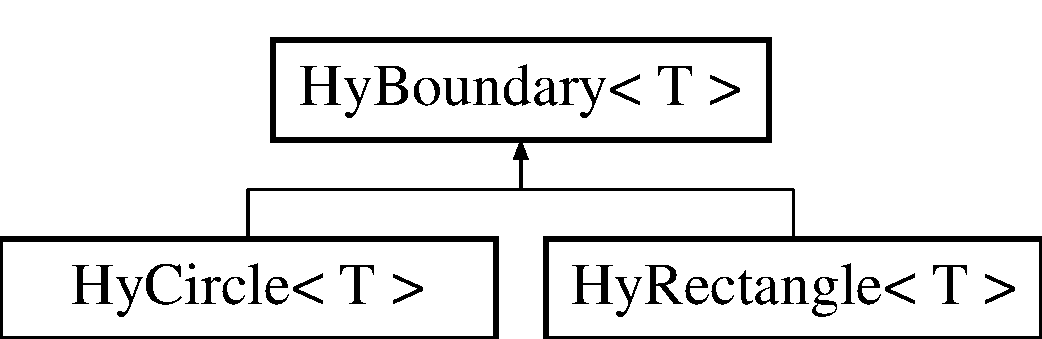
\includegraphics[height=2cm]{classHyBoundary}
\end{center}
\end{figure}
\subsection*{Public Member Functions}
\begin{DoxyCompactItemize}
\item 
\hypertarget{classHyBoundary_aa8cbd9afcca0c5190d485da790a35cb5}{
\hyperlink{classHyBoundary_aa8cbd9afcca0c5190d485da790a35cb5}{HyBoundary} ()}
\label{classHyBoundary_aa8cbd9afcca0c5190d485da790a35cb5}

\begin{DoxyCompactList}\small\item\em Default constructor of \hyperlink{classHyBoundary}{HyBoundary}. \item\end{DoxyCompactList}\item 
\hyperlink{classHyBoundary_a7d47a3c2a01860fa91c754e049e620d5}{HyBoundary} (std::string pDescription)
\begin{DoxyCompactList}\small\item\em Constructor of \hyperlink{classHyBoundary}{HyBoundary}. \item\end{DoxyCompactList}\item 
\hypertarget{classHyBoundary_ad57ad019c8982491f5bcd8270c05d8fc}{
std::string {\bfseries getDescription} () const }
\label{classHyBoundary_ad57ad019c8982491f5bcd8270c05d8fc}

\item 
double \hyperlink{classHyBoundary_a138c96a97075dc41eead25963c1bf785}{getBoundary} (\hyperlink{classHyPoint}{HyPoint}$<$ T $>$ \&pPoint)
\begin{DoxyCompactList}\small\item\em Definition of the boundary. Positive inside the domain, 0 on the boundary, negative outside. \item\end{DoxyCompactList}\item 
\hypertarget{classHyBoundary_aab7edbacd9ab3194cd1704132b040298}{
virtual double {\bfseries getBoundary} (T pX, T pY, T pZ)=0}
\label{classHyBoundary_aab7edbacd9ab3194cd1704132b040298}

\item 
\hyperlink{classHyBoundary}{HyBoundary}$<$ T $>$ \& \hyperlink{classHyBoundary_a0e9c5e3a7b5c161bd47e98ca0e265fc5}{operator=} (const \hyperlink{classHyBoundary}{HyBoundary}$<$ T $>$ \&pB)
\begin{DoxyCompactList}\small\item\em operator= \item\end{DoxyCompactList}\end{DoxyCompactItemize}
\subsection*{Protected Attributes}
\begin{DoxyCompactItemize}
\item 
std::string \hyperlink{classHyBoundary_a0eeb51edf5863746b1f7dbc12c61b1c6}{aDescription}
\end{DoxyCompactItemize}


\subsection{Detailed Description}
\subsubsection*{template$<$typename T$>$ class HyBoundary$<$ T $>$}

Define the border of the domain for a given problem. It is represented by a function, defined in the whole space, which value is positive inside the domain, 0 exactly on the boundary, and negative outside. This class is virtual. 

\subsection{Constructor \& Destructor Documentation}
\hypertarget{classHyBoundary_a7d47a3c2a01860fa91c754e049e620d5}{
\index{HyBoundary@{HyBoundary}!HyBoundary@{HyBoundary}}
\index{HyBoundary@{HyBoundary}!HyBoundary@{HyBoundary}}
\subsubsection[{HyBoundary}]{\setlength{\rightskip}{0pt plus 5cm}template$<$typename T $>$ {\bf HyBoundary}$<$ T $>$::{\bf HyBoundary} (std::string {\em pDescription})\hspace{0.3cm}{\ttfamily  \mbox{[}inline\mbox{]}}}}
\label{classHyBoundary_a7d47a3c2a01860fa91c754e049e620d5}


Constructor of \hyperlink{classHyBoundary}{HyBoundary}. 


\begin{DoxyParams}{Parameters}
\item[{\em pDescription}]Brief description of the boundary. \end{DoxyParams}


\subsection{Member Function Documentation}
\hypertarget{classHyBoundary_a138c96a97075dc41eead25963c1bf785}{
\index{HyBoundary@{HyBoundary}!getBoundary@{getBoundary}}
\index{getBoundary@{getBoundary}!HyBoundary@{HyBoundary}}
\subsubsection[{getBoundary}]{\setlength{\rightskip}{0pt plus 5cm}template$<$typename T $>$ double {\bf HyBoundary}$<$ T $>$::getBoundary ({\bf HyPoint}$<$ T $>$ \& {\em pPoint})\hspace{0.3cm}{\ttfamily  \mbox{[}inline\mbox{]}}}}
\label{classHyBoundary_a138c96a97075dc41eead25963c1bf785}


Definition of the boundary. Positive inside the domain, 0 on the boundary, negative outside. 


\begin{DoxyParams}{Parameters}
\item[{\em pPoint}]The point to evalutate. \end{DoxyParams}


Reimplemented in \hyperlink{classHyCircle_aed6e84c3e2e99b8f84aa1b723224f4c5}{HyCircle$<$ T $>$}, and \hyperlink{classHyRectangle_a881f7ed847a94d1af3ff4ff0d60ee516}{HyRectangle$<$ T $>$}.

\hypertarget{classHyBoundary_a0e9c5e3a7b5c161bd47e98ca0e265fc5}{
\index{HyBoundary@{HyBoundary}!operator=@{operator=}}
\index{operator=@{operator=}!HyBoundary@{HyBoundary}}
\subsubsection[{operator=}]{\setlength{\rightskip}{0pt plus 5cm}template$<$typename T $>$ {\bf HyBoundary}$<$ T $>$ \& {\bf HyBoundary}$<$ T $>$::operator= (const {\bf HyBoundary}$<$ T $>$ \& {\em pB})\hspace{0.3cm}{\ttfamily  \mbox{[}inline\mbox{]}}}}
\label{classHyBoundary_a0e9c5e3a7b5c161bd47e98ca0e265fc5}


operator= 


\begin{DoxyParams}{Parameters}
\item[{\em pB}]The \hyperlink{classHyBoundary}{HyBoundary} to copy. \end{DoxyParams}


\subsection{Member Data Documentation}
\hypertarget{classHyBoundary_a0eeb51edf5863746b1f7dbc12c61b1c6}{
\index{HyBoundary@{HyBoundary}!aDescription@{aDescription}}
\index{aDescription@{aDescription}!HyBoundary@{HyBoundary}}
\subsubsection[{aDescription}]{\setlength{\rightskip}{0pt plus 5cm}template$<$typename T$>$ std::string {\bf HyBoundary}$<$ T $>$::{\bf aDescription}\hspace{0.3cm}{\ttfamily  \mbox{[}protected\mbox{]}}}}
\label{classHyBoundary_a0eeb51edf5863746b1f7dbc12c61b1c6}
A brief description of the boundary 

The documentation for this class was generated from the following files:\begin{DoxyCompactItemize}
\item 
\hyperlink{HyBoundary_8hpp}{HyBoundary.hpp}\item 
\hyperlink{HyBoundary_8ipp}{HyBoundary.ipp}\end{DoxyCompactItemize}

\hypertarget{classHyCircle}{
\section{HyCircle$<$ T $>$ Class Template Reference}
\label{classHyCircle}\index{HyCircle@{HyCircle}}
}
Inheritance diagram for HyCircle$<$ T $>$:\begin{figure}[H]
\begin{center}
\leavevmode
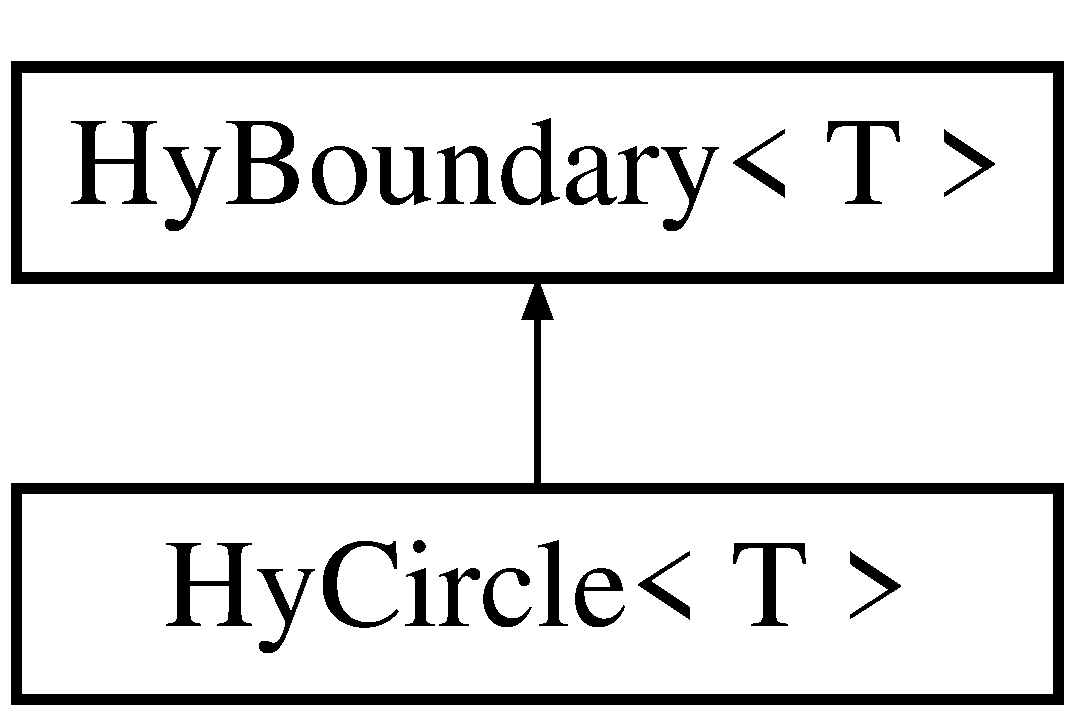
\includegraphics[height=2cm]{classHyCircle}
\end{center}
\end{figure}
\subsection*{Public Member Functions}
\begin{DoxyCompactItemize}
\item 
\hypertarget{classHyCircle_adc55ea1795d45073c90c462bda267e6f}{
{\bfseries HyCircle} (double pRadius, \hyperlink{classHyPoint}{HyPoint}$<$ T $>$ \&pP)}
\label{classHyCircle_adc55ea1795d45073c90c462bda267e6f}

\item 
\hypertarget{classHyCircle_aa730543a6c7b464024fc530cf49e3c28}{
double {\bfseries getRadius} ()}
\label{classHyCircle_aa730543a6c7b464024fc530cf49e3c28}

\item 
\hypertarget{classHyCircle_a06295a19bea9a4afef499d10b7edb5fd}{
\hyperlink{classHyPoint}{HyPoint}$<$ T $>$ \& {\bfseries getCenter} ()}
\label{classHyCircle_a06295a19bea9a4afef499d10b7edb5fd}

\item 
\hypertarget{classHyCircle_a47d49ab084e13d1af2f6b8b7d8d3fdc0}{
void {\bfseries setRadius} (double pRadius)}
\label{classHyCircle_a47d49ab084e13d1af2f6b8b7d8d3fdc0}

\item 
\hypertarget{classHyCircle_a69ada2f6b472a1f1f7ecefa0d94210ec}{
void {\bfseries setCenter} (\hyperlink{classHyPoint}{HyPoint}$<$ T $>$ \&pCenter)}
\label{classHyCircle_a69ada2f6b472a1f1f7ecefa0d94210ec}

\item 
double \hyperlink{classHyCircle_aed6e84c3e2e99b8f84aa1b723224f4c5}{getBoundary} (\hyperlink{classHyPoint}{HyPoint}$<$ T $>$ \&pPoint)
\begin{DoxyCompactList}\small\item\em Definition of the boundary. Positive inside the domain, 0 on the boundary, negative outside. \item\end{DoxyCompactList}\item 
\hypertarget{classHyCircle_a08ababcaa26c11288e66a66a3d0e7f38}{
double {\bfseries getBoundary} (T pX, T pY, T pZ)}
\label{classHyCircle_a08ababcaa26c11288e66a66a3d0e7f38}

\item 
\hypertarget{classHyCircle_aeed0b7d097fbd97cfe87c8f7dc4e0b52}{
\hyperlink{classHyCircle}{HyCircle}$<$ T $>$ \& {\bfseries operator=} (const \hyperlink{classHyCircle}{HyCircle}$<$ T $>$ \&pC)}
\label{classHyCircle_aeed0b7d097fbd97cfe87c8f7dc4e0b52}

\end{DoxyCompactItemize}
\subsection*{Protected Attributes}
\begin{DoxyCompactItemize}
\item 
\hypertarget{classHyCircle_a7df9d0c4404401ba9f661aad0bd7bc6e}{
double {\bfseries aRadius}}
\label{classHyCircle_a7df9d0c4404401ba9f661aad0bd7bc6e}

\item 
\hypertarget{classHyCircle_adf84a8e946e0fb915d313ba0051c5b23}{
\hyperlink{classHyPoint}{HyPoint}$<$ T $>$ {\bfseries aCenter}}
\label{classHyCircle_adf84a8e946e0fb915d313ba0051c5b23}

\end{DoxyCompactItemize}
\subsubsection*{template$<$typename T$>$ class HyCircle$<$ T $>$}



\subsection{Member Function Documentation}
\hypertarget{classHyCircle_aed6e84c3e2e99b8f84aa1b723224f4c5}{
\index{HyCircle@{HyCircle}!getBoundary@{getBoundary}}
\index{getBoundary@{getBoundary}!HyCircle@{HyCircle}}
\subsubsection[{getBoundary}]{\setlength{\rightskip}{0pt plus 5cm}template$<$typename T $>$ double {\bf HyCircle}$<$ T $>$::getBoundary ({\bf HyPoint}$<$ T $>$ \& {\em pPoint})\hspace{0.3cm}{\ttfamily  \mbox{[}inline\mbox{]}}}}
\label{classHyCircle_aed6e84c3e2e99b8f84aa1b723224f4c5}


Definition of the boundary. Positive inside the domain, 0 on the boundary, negative outside. 


\begin{DoxyParams}{Parameters}
\item[{\em pPoint}]The point to evalutate. \end{DoxyParams}


Reimplemented from \hyperlink{classHyBoundary_a138c96a97075dc41eead25963c1bf785}{HyBoundary$<$ T $>$}.



The documentation for this class was generated from the following files:\begin{DoxyCompactItemize}
\item 
HyCircle.hpp\item 
HyCircle.ipp\end{DoxyCompactItemize}

\hypertarget{classHyDiffusion2D}{
\section{HyDiffusion2D$<$ T $>$ Class Template Reference}
\label{classHyDiffusion2D}\index{HyDiffusion2D@{HyDiffusion2D}}
}


Diffusion equation in 2 dimensions: $ \partial_t u - \kappa\Delta u = f $.  




{\ttfamily \#include $<$HyDiffusion2D.hpp$>$}

Inheritance diagram for HyDiffusion2D$<$ T $>$:\begin{figure}[H]
\begin{center}
\leavevmode
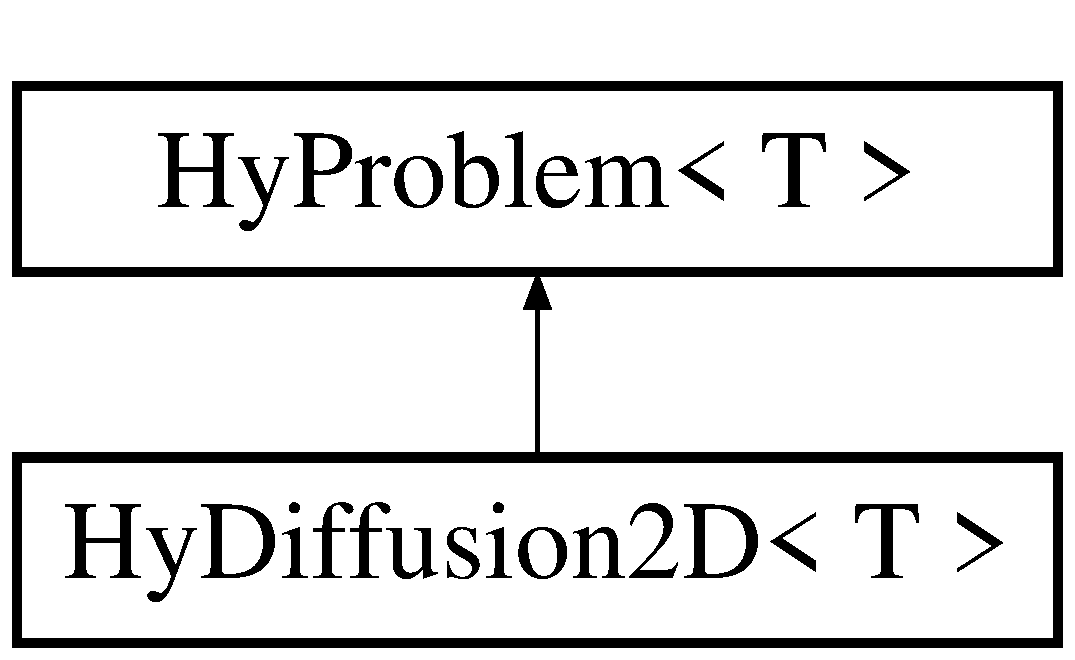
\includegraphics[height=2cm]{classHyDiffusion2D}
\end{center}
\end{figure}
\subsection*{Public Member Functions}
\begin{DoxyCompactItemize}
\item 
\hypertarget{classHyDiffusion2D_aab727755e5fd2fe558b1405b7286d80c}{
\hyperlink{classHyDiffusion2D_aab727755e5fd2fe558b1405b7286d80c}{HyDiffusion2D} ()}
\label{classHyDiffusion2D_aab727755e5fd2fe558b1405b7286d80c}

\begin{DoxyCompactList}\small\item\em Default constructor. \item\end{DoxyCompactList}\item 
\hypertarget{classHyDiffusion2D_a3e7c4a79c2a9bc64749caf72c876719c}{
{\bfseries HyDiffusion2D} (\hyperlink{classHyDomain}{HyDomain}$<$ T $>$ \&pDomain, \hyperlink{classHyBoundary}{HyBoundary}$<$ T $>$ \&pBoundary, \hyperlink{classHyMesh2D}{HyMesh2D}$<$ T $>$ \&pMesh, std::string \&pDescription, long int pTmax, unsigned long int pNbTimeStep=1, double pK=1)}
\label{classHyDiffusion2D_a3e7c4a79c2a9bc64749caf72c876719c}

\item 
\hypertarget{classHyDiffusion2D_a6bb3997b896afa965dab984f39e85adb}{
std::vector$<$ Eigen::VectorXd $>$ {\bfseries getEvolution} () const }
\label{classHyDiffusion2D_a6bb3997b896afa965dab984f39e85adb}

\item 
\hypertarget{classHyDiffusion2D_a8a6f0ed50d0e2523a6998457b4607b17}{
void \hyperlink{classHyDiffusion2D_a8a6f0ed50d0e2523a6998457b4607b17}{build} ()}
\label{classHyDiffusion2D_a8a6f0ed50d0e2523a6998457b4607b17}

\begin{DoxyCompactList}\small\item\em Fills the matrix A and the vectors F and G. \item\end{DoxyCompactList}\item 
\hypertarget{classHyDiffusion2D_a7f66b2d5a7ddafa4da4d100219ff2073}{
void {\bfseries buildTheta} (double pTheta)}
\label{classHyDiffusion2D_a7f66b2d5a7ddafa4da4d100219ff2073}

\item 
\hypertarget{classHyDiffusion2D_a8d6bbc8e9c91c4eaf7215e14d6504af6}{
void \hyperlink{classHyDiffusion2D_a8d6bbc8e9c91c4eaf7215e14d6504af6}{solve} ()}
\label{classHyDiffusion2D_a8d6bbc8e9c91c4eaf7215e14d6504af6}

\begin{DoxyCompactList}\small\item\em Solve the problem using the explicit method by default. \item\end{DoxyCompactList}\item 
\hypertarget{classHyDiffusion2D_a68af2c8f0a1fa5de0589997c8287b8db}{
void \hyperlink{classHyDiffusion2D_a68af2c8f0a1fa5de0589997c8287b8db}{solveExplicit} ()}
\label{classHyDiffusion2D_a68af2c8f0a1fa5de0589997c8287b8db}

\begin{DoxyCompactList}\small\item\em Solve the problem using the explicit method. \item\end{DoxyCompactList}\item 
\hypertarget{classHyDiffusion2D_ae5b91bf3392c29384651599d8d115284}{
void {\bfseries solveTheta} ()}
\label{classHyDiffusion2D_ae5b91bf3392c29384651599d8d115284}

\item 
void \hyperlink{classHyDiffusion2D_a88da599f17d9a34ee45526cf8beffa54}{displaySolutionGP} (std::ostream \&out, unsigned long int t)
\begin{DoxyCompactList}\small\item\em Display the solution for gnuplot, using the pattern \char`\"{}X Y VALUE\char`\"{} (to display in 3D). \item\end{DoxyCompactList}\item 
double \hyperlink{classHyDiffusion2D_a0df1a7fbe0b6a50d85a74c655f32cfb2}{g} (\hyperlink{classHyPoint}{HyPoint}$<$ T $>$ pPoint)
\begin{DoxyCompactList}\small\item\em Dirichlet condition. \item\end{DoxyCompactList}\item 
double \hyperlink{classHyDiffusion2D_ae09f11a685b241e42b466d023b1d23fc}{g} (T pX, T pY, T pZ)
\begin{DoxyCompactList}\small\item\em Dirichlet condition. \item\end{DoxyCompactList}\item 
double \hyperlink{classHyDiffusion2D_a40c7ec43e3b5e0d1d1d518dabd3a2299}{f} (\hyperlink{classHyPoint}{HyPoint}$<$ T $>$ pPoint)
\begin{DoxyCompactList}\small\item\em The function f of the Diffusion equation. \item\end{DoxyCompactList}\item 
double \hyperlink{classHyDiffusion2D_aea84648a2e7b70f9eda67ef603102a11}{f} (T pX, T pY)
\begin{DoxyCompactList}\small\item\em The function f of the Diffusion equation. \item\end{DoxyCompactList}\item 
double \hyperlink{classHyDiffusion2D_a07622cf68cbd0571101807eedcb3a76d}{initialCondition} (\hyperlink{classHyPoint}{HyPoint}$<$ T $>$ pPoint)
\begin{DoxyCompactList}\small\item\em The initial condition. \item\end{DoxyCompactList}\item 
double \hyperlink{classHyDiffusion2D_ae04d50ba468b2338bbf4d134d43ffe49}{initialCondition} (T pX, T pY)
\begin{DoxyCompactList}\small\item\em The initial condition. \item\end{DoxyCompactList}\end{DoxyCompactItemize}
\subsection*{Protected Attributes}
\begin{DoxyCompactItemize}
\item 
long int \hyperlink{classHyDiffusion2D_a484433cb70b279d460ae7ad99c692b44}{aTmax}
\item 
unsigned long int \hyperlink{classHyDiffusion2D_a3fdb9b91352535d51ab737c8e2bbb096}{aNbTimeStep}
\item 
double \hyperlink{classHyDiffusion2D_adb712ad9fbd8ff8ba019bd0a5c80edb4}{aK}
\item 
Eigen::SparseMatrix$<$ T $>$ \hyperlink{classHyDiffusion2D_a3826559f9dade45395fc0bb046fbab9c}{aMatrixB}
\item 
std::vector$<$ Eigen::VectorXd $>$ \hyperlink{classHyDiffusion2D_aaba7bf56f39cc0caa9bcf8fa4b2f30f0}{aEvolution}
\end{DoxyCompactItemize}


\subsection{Detailed Description}
\subsubsection*{template$<$typename T$>$ class HyDiffusion2D$<$ T $>$}

Diffusion equation in 2 dimensions: $ \partial_t u - \kappa\Delta u = f $. 

\subsection{Member Function Documentation}
\hypertarget{classHyDiffusion2D_a88da599f17d9a34ee45526cf8beffa54}{
\index{HyDiffusion2D@{HyDiffusion2D}!displaySolutionGP@{displaySolutionGP}}
\index{displaySolutionGP@{displaySolutionGP}!HyDiffusion2D@{HyDiffusion2D}}
\subsubsection[{displaySolutionGP}]{\setlength{\rightskip}{0pt plus 5cm}template$<$typename T $>$ void {\bf HyDiffusion2D}$<$ T $>$::displaySolutionGP (std::ostream \& {\em out}, \/  unsigned long int {\em t})\hspace{0.3cm}{\ttfamily  \mbox{[}inline\mbox{]}}}}
\label{classHyDiffusion2D_a88da599f17d9a34ee45526cf8beffa54}


Display the solution for gnuplot, using the pattern \char`\"{}X Y VALUE\char`\"{} (to display in 3D). 


\begin{DoxyParams}{Parameters}
\item[{\em out}]The ostream to write in \item[{\em t}]The time of evolution \end{DoxyParams}
\hypertarget{classHyDiffusion2D_aea84648a2e7b70f9eda67ef603102a11}{
\index{HyDiffusion2D@{HyDiffusion2D}!f@{f}}
\index{f@{f}!HyDiffusion2D@{HyDiffusion2D}}
\subsubsection[{f}]{\setlength{\rightskip}{0pt plus 5cm}template$<$typename T $>$ double {\bf HyDiffusion2D}$<$ T $>$::f (T {\em pX}, \/  T {\em pY})\hspace{0.3cm}{\ttfamily  \mbox{[}inline\mbox{]}}}}
\label{classHyDiffusion2D_aea84648a2e7b70f9eda67ef603102a11}


The function f of the Diffusion equation. 


\begin{DoxyParams}{Parameters}
\item[{\em pX,pY}]The coordinate of evaluation \end{DoxyParams}
\begin{DoxyReturn}{Returns}
The value of f(pX,pY) 
\end{DoxyReturn}
\hypertarget{classHyDiffusion2D_a40c7ec43e3b5e0d1d1d518dabd3a2299}{
\index{HyDiffusion2D@{HyDiffusion2D}!f@{f}}
\index{f@{f}!HyDiffusion2D@{HyDiffusion2D}}
\subsubsection[{f}]{\setlength{\rightskip}{0pt plus 5cm}template$<$typename T $>$ double {\bf HyDiffusion2D}$<$ T $>$::f ({\bf HyPoint}$<$ T $>$ {\em pPoint})\hspace{0.3cm}{\ttfamily  \mbox{[}inline\mbox{]}}}}
\label{classHyDiffusion2D_a40c7ec43e3b5e0d1d1d518dabd3a2299}


The function f of the Diffusion equation. 


\begin{DoxyParams}{Parameters}
\item[{\em pPoint}]The point of evaluation \end{DoxyParams}
\begin{DoxyReturn}{Returns}
The value of f(pPoint) 
\end{DoxyReturn}
\hypertarget{classHyDiffusion2D_ae09f11a685b241e42b466d023b1d23fc}{
\index{HyDiffusion2D@{HyDiffusion2D}!g@{g}}
\index{g@{g}!HyDiffusion2D@{HyDiffusion2D}}
\subsubsection[{g}]{\setlength{\rightskip}{0pt plus 5cm}template$<$typename T $>$ double {\bf HyDiffusion2D}$<$ T $>$::g (T {\em pX}, \/  T {\em pY}, \/  T {\em pZ})\hspace{0.3cm}{\ttfamily  \mbox{[}inline\mbox{]}}}}
\label{classHyDiffusion2D_ae09f11a685b241e42b466d023b1d23fc}


Dirichlet condition. 


\begin{DoxyParams}{Parameters}
\item[{\em pX,pY,pZ}]The coordinates of evaluation \end{DoxyParams}
\begin{DoxyReturn}{Returns}
The value of the Dirichlet condition for the given point (pX,pY,pZ) 
\end{DoxyReturn}


Reimplemented from \hyperlink{classHyProblem}{HyProblem$<$ T $>$}.

\hypertarget{classHyDiffusion2D_a0df1a7fbe0b6a50d85a74c655f32cfb2}{
\index{HyDiffusion2D@{HyDiffusion2D}!g@{g}}
\index{g@{g}!HyDiffusion2D@{HyDiffusion2D}}
\subsubsection[{g}]{\setlength{\rightskip}{0pt plus 5cm}template$<$typename T $>$ double {\bf HyDiffusion2D}$<$ T $>$::g ({\bf HyPoint}$<$ T $>$ {\em pPoint})\hspace{0.3cm}{\ttfamily  \mbox{[}inline\mbox{]}}}}
\label{classHyDiffusion2D_a0df1a7fbe0b6a50d85a74c655f32cfb2}


Dirichlet condition. 


\begin{DoxyParams}{Parameters}
\item[{\em pPoint}]The point to evaluate \end{DoxyParams}
\begin{DoxyReturn}{Returns}
The value of the Dirichlet condition for the given point 
\end{DoxyReturn}


Reimplemented from \hyperlink{classHyProblem_a5d3b78c69811136e74e9fc9232cc110b}{HyProblem$<$ T $>$}.

\hypertarget{classHyDiffusion2D_ae04d50ba468b2338bbf4d134d43ffe49}{
\index{HyDiffusion2D@{HyDiffusion2D}!initialCondition@{initialCondition}}
\index{initialCondition@{initialCondition}!HyDiffusion2D@{HyDiffusion2D}}
\subsubsection[{initialCondition}]{\setlength{\rightskip}{0pt plus 5cm}template$<$typename T $>$ double {\bf HyDiffusion2D}$<$ T $>$::initialCondition (T {\em pX}, \/  T {\em pY})\hspace{0.3cm}{\ttfamily  \mbox{[}inline\mbox{]}}}}
\label{classHyDiffusion2D_ae04d50ba468b2338bbf4d134d43ffe49}


The initial condition. 


\begin{DoxyParams}{Parameters}
\item[{\em pX,pY}]The coordinate of evaluation \end{DoxyParams}
\begin{DoxyReturn}{Returns}
The value of f(pX,pY) 
\end{DoxyReturn}
\hypertarget{classHyDiffusion2D_a07622cf68cbd0571101807eedcb3a76d}{
\index{HyDiffusion2D@{HyDiffusion2D}!initialCondition@{initialCondition}}
\index{initialCondition@{initialCondition}!HyDiffusion2D@{HyDiffusion2D}}
\subsubsection[{initialCondition}]{\setlength{\rightskip}{0pt plus 5cm}template$<$typename T $>$ double {\bf HyDiffusion2D}$<$ T $>$::initialCondition ({\bf HyPoint}$<$ T $>$ {\em pPoint})\hspace{0.3cm}{\ttfamily  \mbox{[}inline\mbox{]}}}}
\label{classHyDiffusion2D_a07622cf68cbd0571101807eedcb3a76d}


The initial condition. 


\begin{DoxyParams}{Parameters}
\item[{\em pPoint}]The point of evaluation \end{DoxyParams}
\begin{DoxyReturn}{Returns}
The value of f(pPoint) 
\end{DoxyReturn}


\subsection{Member Data Documentation}
\hypertarget{classHyDiffusion2D_aaba7bf56f39cc0caa9bcf8fa4b2f30f0}{
\index{HyDiffusion2D@{HyDiffusion2D}!aEvolution@{aEvolution}}
\index{aEvolution@{aEvolution}!HyDiffusion2D@{HyDiffusion2D}}
\subsubsection[{aEvolution}]{\setlength{\rightskip}{0pt plus 5cm}template$<$typename T $>$ std::vector$<$Eigen::VectorXd$>$ {\bf HyDiffusion2D}$<$ T $>$::{\bf aEvolution}\hspace{0.3cm}{\ttfamily  \mbox{[}protected\mbox{]}}}}
\label{classHyDiffusion2D_aaba7bf56f39cc0caa9bcf8fa4b2f30f0}
The set of all solution for each time step \hypertarget{classHyDiffusion2D_adb712ad9fbd8ff8ba019bd0a5c80edb4}{
\index{HyDiffusion2D@{HyDiffusion2D}!aK@{aK}}
\index{aK@{aK}!HyDiffusion2D@{HyDiffusion2D}}
\subsubsection[{aK}]{\setlength{\rightskip}{0pt plus 5cm}template$<$typename T $>$ double {\bf HyDiffusion2D}$<$ T $>$::{\bf aK}\hspace{0.3cm}{\ttfamily  \mbox{[}protected\mbox{]}}}}
\label{classHyDiffusion2D_adb712ad9fbd8ff8ba019bd0a5c80edb4}
The diffusion coefficient \hypertarget{classHyDiffusion2D_a3826559f9dade45395fc0bb046fbab9c}{
\index{HyDiffusion2D@{HyDiffusion2D}!aMatrixB@{aMatrixB}}
\index{aMatrixB@{aMatrixB}!HyDiffusion2D@{HyDiffusion2D}}
\subsubsection[{aMatrixB}]{\setlength{\rightskip}{0pt plus 5cm}template$<$typename T $>$ Eigen::SparseMatrix$<$T$>$ {\bf HyDiffusion2D}$<$ T $>$::{\bf aMatrixB}\hspace{0.3cm}{\ttfamily  \mbox{[}protected\mbox{]}}}}
\label{classHyDiffusion2D_a3826559f9dade45395fc0bb046fbab9c}
The matrix B for the theta method ( A x(n+1) = B x(n) + F + G ) \hypertarget{classHyDiffusion2D_a3fdb9b91352535d51ab737c8e2bbb096}{
\index{HyDiffusion2D@{HyDiffusion2D}!aNbTimeStep@{aNbTimeStep}}
\index{aNbTimeStep@{aNbTimeStep}!HyDiffusion2D@{HyDiffusion2D}}
\subsubsection[{aNbTimeStep}]{\setlength{\rightskip}{0pt plus 5cm}template$<$typename T $>$ unsigned long int {\bf HyDiffusion2D}$<$ T $>$::{\bf aNbTimeStep}\hspace{0.3cm}{\ttfamily  \mbox{[}protected\mbox{]}}}}
\label{classHyDiffusion2D_a3fdb9b91352535d51ab737c8e2bbb096}
The number of temporal steps \hypertarget{classHyDiffusion2D_a484433cb70b279d460ae7ad99c692b44}{
\index{HyDiffusion2D@{HyDiffusion2D}!aTmax@{aTmax}}
\index{aTmax@{aTmax}!HyDiffusion2D@{HyDiffusion2D}}
\subsubsection[{aTmax}]{\setlength{\rightskip}{0pt plus 5cm}template$<$typename T $>$ long int {\bf HyDiffusion2D}$<$ T $>$::{\bf aTmax}\hspace{0.3cm}{\ttfamily  \mbox{[}protected\mbox{]}}}}
\label{classHyDiffusion2D_a484433cb70b279d460ae7ad99c692b44}
The maximal time 

The documentation for this class was generated from the following files:\begin{DoxyCompactItemize}
\item 
\hyperlink{HyDiffusion2D_8hpp}{HyDiffusion2D.hpp}\item 
\hyperlink{HyDiffusion2D_8ipp}{HyDiffusion2D.ipp}\end{DoxyCompactItemize}

\hypertarget{classHyDomain}{
\section{HyDomain$<$ T $>$ Class Template Reference}
\label{classHyDomain}\index{HyDomain@{HyDomain}}
}
\subsection*{Public Member Functions}
\begin{DoxyCompactItemize}
\item 
\hypertarget{classHyDomain_a78c1bc2d22889c85bbfc97fc9a5c7f47}{
{\bfseries HyDomain} (const \hyperlink{classHyDomain}{HyDomain} \&pDomain)}
\label{classHyDomain_a78c1bc2d22889c85bbfc97fc9a5c7f47}

\item 
\hypertarget{classHyDomain_af225dd17835a2edfabf1ac0a71e29100}{
{\bfseries HyDomain} (\hyperlink{classHyPoint}{HyPoint}$<$ T $>$ pBL, \hyperlink{classHyPoint}{HyPoint}$<$ T $>$ pUR)}
\label{classHyDomain_af225dd17835a2edfabf1ac0a71e29100}

\item 
\hypertarget{classHyDomain_a80dc12dbe00d07a91176c8e0b6d4279d}{
\hyperlink{classHyPoint}{HyPoint}$<$ T $>$ \& {\bfseries getBL} ()}
\label{classHyDomain_a80dc12dbe00d07a91176c8e0b6d4279d}

\item 
\hypertarget{classHyDomain_aaf438198d089dcead1a695da5527e5e3}{
\hyperlink{classHyPoint}{HyPoint}$<$ T $>$ \& {\bfseries getUR} ()}
\label{classHyDomain_aaf438198d089dcead1a695da5527e5e3}

\end{DoxyCompactItemize}
\subsection*{Protected Attributes}
\begin{DoxyCompactItemize}
\item 
\hypertarget{classHyDomain_ad9d2958f0843f21478075c8f7547d486}{
\hyperlink{classHyPoint}{HyPoint}$<$ T $>$ {\bfseries aBL}}
\label{classHyDomain_ad9d2958f0843f21478075c8f7547d486}

\item 
\hypertarget{classHyDomain_a6423102e3c063a7c5b5202e4a1b35a2f}{
\hyperlink{classHyPoint}{HyPoint}$<$ T $>$ {\bfseries aUR}}
\label{classHyDomain_a6423102e3c063a7c5b5202e4a1b35a2f}

\end{DoxyCompactItemize}
\subsubsection*{template$<$typename T$>$ class HyDomain$<$ T $>$}



The documentation for this class was generated from the following files:\begin{DoxyCompactItemize}
\item 
HyDomain.hpp\item 
HyDomain.ipp\end{DoxyCompactItemize}

\hypertarget{classHyMesh}{
\section{HyMesh$<$ T $>$ Class Template Reference}
\label{classHyMesh}\index{HyMesh@{HyMesh}}
}
Inheritance diagram for HyMesh$<$ T $>$:\begin{figure}[H]
\begin{center}
\leavevmode
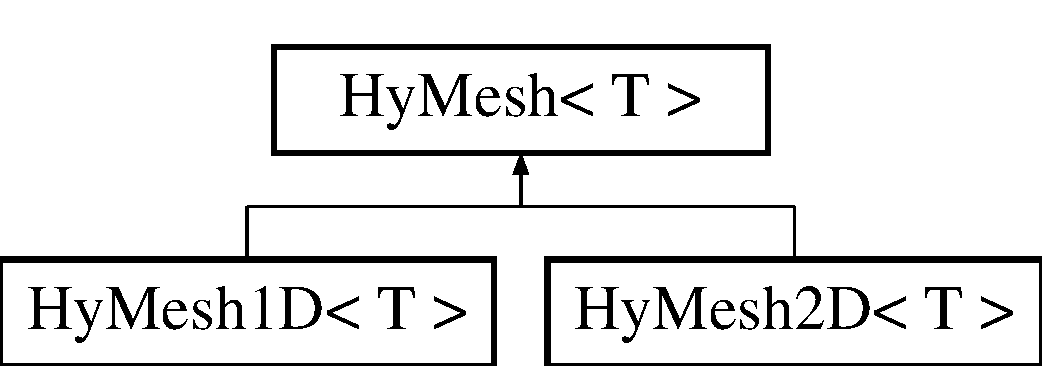
\includegraphics[height=2cm]{classHyMesh}
\end{center}
\end{figure}
\subsection*{Public Member Functions}
\begin{DoxyCompactItemize}
\item 
\hypertarget{classHyMesh_a45186552fa4dae91f6e9bbd4237d85a9}{
unsigned int {\bfseries getDimension} ()}
\label{classHyMesh_a45186552fa4dae91f6e9bbd4237d85a9}

\item 
\hypertarget{classHyMesh_a1d72d00c1ff7bf98d9d18eafdf729b69}{
virtual void {\bfseries display} ()=0}
\label{classHyMesh_a1d72d00c1ff7bf98d9d18eafdf729b69}

\end{DoxyCompactItemize}
\subsection*{Protected Attributes}
\begin{DoxyCompactItemize}
\item 
\hypertarget{classHyMesh_ae1a78ec74b87c3646d2e9cad978546f8}{
unsigned int {\bfseries aDimension}}
\label{classHyMesh_ae1a78ec74b87c3646d2e9cad978546f8}

\end{DoxyCompactItemize}
\subsubsection*{template$<$typename T$>$ class HyMesh$<$ T $>$}



The documentation for this class was generated from the following files:\begin{DoxyCompactItemize}
\item 
HyMesh.hpp\item 
HyMesh.ipp\end{DoxyCompactItemize}

\hypertarget{classHyMesh1D}{
\section{HyMesh1D$<$ T $>$ Class Template Reference}
\label{classHyMesh1D}\index{HyMesh1D@{HyMesh1D}}
}
Inheritance diagram for HyMesh1D$<$ T $>$:\begin{figure}[H]
\begin{center}
\leavevmode
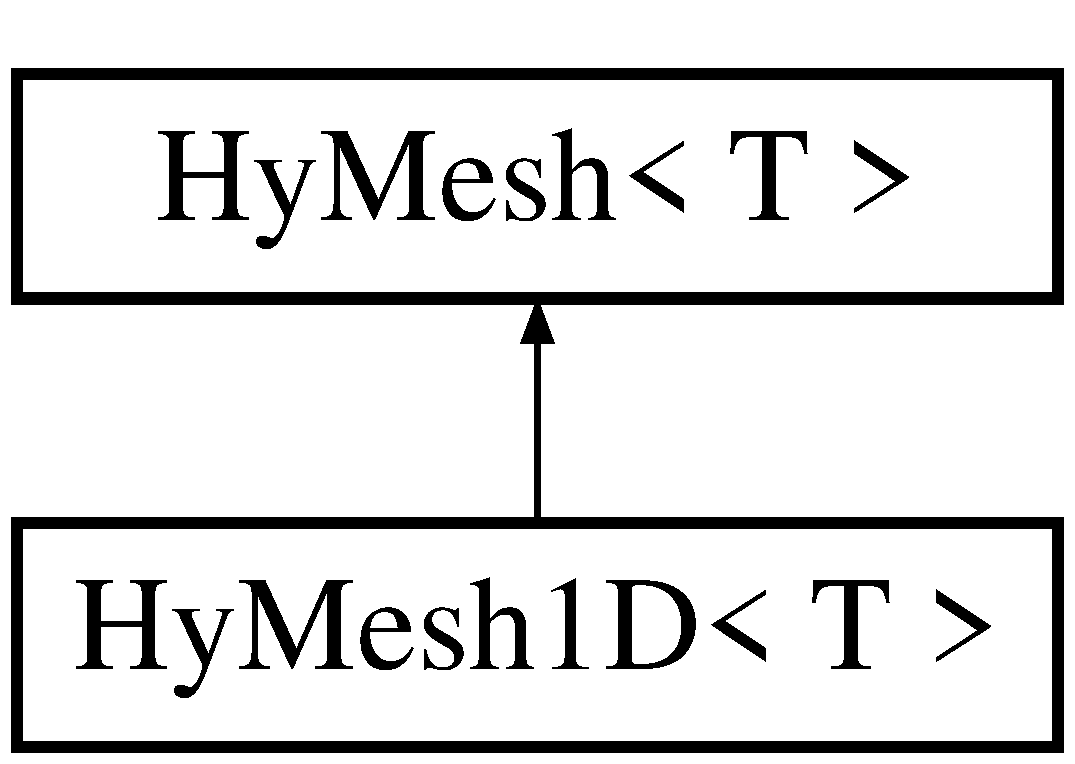
\includegraphics[height=2cm]{classHyMesh1D}
\end{center}
\end{figure}
\subsection*{Public Member Functions}
\begin{DoxyCompactItemize}
\item 
\hypertarget{classHyMesh1D_a7bfabb4cb61760a439ffd07c42150c53}{
{\bfseries HyMesh1D} (\hyperlink{classHyPoint}{HyPoint}$<$ T $>$ \&pBL, \hyperlink{classHyPoint}{HyPoint}$<$ T $>$ \&pUR, unsigned long pNbRectanglesX)}
\label{classHyMesh1D_a7bfabb4cb61760a439ffd07c42150c53}

\item 
\hypertarget{classHyMesh1D_aba7a70a7db8172726f77eca7d72a5b97}{
{\bfseries HyMesh1D} (\hyperlink{classHyMesh1D}{HyMesh1D}$<$ T $>$ \&pMesh)}
\label{classHyMesh1D_aba7a70a7db8172726f77eca7d72a5b97}

\item 
\hypertarget{classHyMesh1D_aae6435a1ffbdd95de5b67620eec79e81}{
std::vector$<$ \hyperlink{classHyPoint}{HyPoint}$<$ T $>$ $>$ {\bfseries getMesh} ()}
\label{classHyMesh1D_aae6435a1ffbdd95de5b67620eec79e81}

\item 
\hypertarget{classHyMesh1D_a7c6d73f2ca7f4b92fad7aed304e5fb62}{
unsigned long {\bfseries getNbRectanglesX} ()}
\label{classHyMesh1D_a7c6d73f2ca7f4b92fad7aed304e5fb62}

\item 
\hypertarget{classHyMesh1D_a2c34467214ad7b0bf1070f4e6e90e446}{
double {\bfseries getHX} ()}
\label{classHyMesh1D_a2c34467214ad7b0bf1070f4e6e90e446}

\item 
\hypertarget{classHyMesh1D_a4fbd824ebe60ba0c844441e8de7e53b0}{
unsigned long {\bfseries size} ()}
\label{classHyMesh1D_a4fbd824ebe60ba0c844441e8de7e53b0}

\item 
\hypertarget{classHyMesh1D_abb7bc7c5d83046745958a8b2f0accd59}{
\hyperlink{classHyPoint}{HyPoint}$<$ T $>$ \& {\bfseries operator\mbox{[}$\,$\mbox{]}} (unsigned long i)}
\label{classHyMesh1D_abb7bc7c5d83046745958a8b2f0accd59}

\item 
\hypertarget{classHyMesh1D_a3a5fd4c05d03c6e45293a34a0d112114}{
void {\bfseries display} ()}
\label{classHyMesh1D_a3a5fd4c05d03c6e45293a34a0d112114}

\end{DoxyCompactItemize}
\subsection*{Protected Attributes}
\begin{DoxyCompactItemize}
\item 
\hypertarget{classHyMesh1D_a4518a7522f676f60cdb291cd293db150}{
std::vector$<$ \hyperlink{classHyPoint}{HyPoint}$<$ T $>$ $>$ {\bfseries aMesh}}
\label{classHyMesh1D_a4518a7522f676f60cdb291cd293db150}

\item 
\hypertarget{classHyMesh1D_a89436efe296366f4373d29587b6acc49}{
unsigned long {\bfseries aNbRectanglesX}}
\label{classHyMesh1D_a89436efe296366f4373d29587b6acc49}

\item 
\hypertarget{classHyMesh1D_a3f97f02064dc0c71d53cc62ed13ba1f5}{
double {\bfseries ahX}}
\label{classHyMesh1D_a3f97f02064dc0c71d53cc62ed13ba1f5}

\end{DoxyCompactItemize}
\subsubsection*{template$<$typename T$>$ class HyMesh1D$<$ T $>$}



The documentation for this class was generated from the following files:\begin{DoxyCompactItemize}
\item 
\hyperlink{HyMesh1D_8hpp}{HyMesh1D.hpp}\item 
HyMesh1D.ipp\end{DoxyCompactItemize}

\hypertarget{classHyMesh2D}{
\section{HyMesh2D$<$ T $>$ Class Template Reference}
\label{classHyMesh2D}\index{HyMesh2D@{HyMesh2D}}
}


Two dimensional mesh.  




{\ttfamily \#include $<$HyMesh2D.hpp$>$}

Inheritance diagram for HyMesh2D$<$ T $>$:\begin{figure}[H]
\begin{center}
\leavevmode
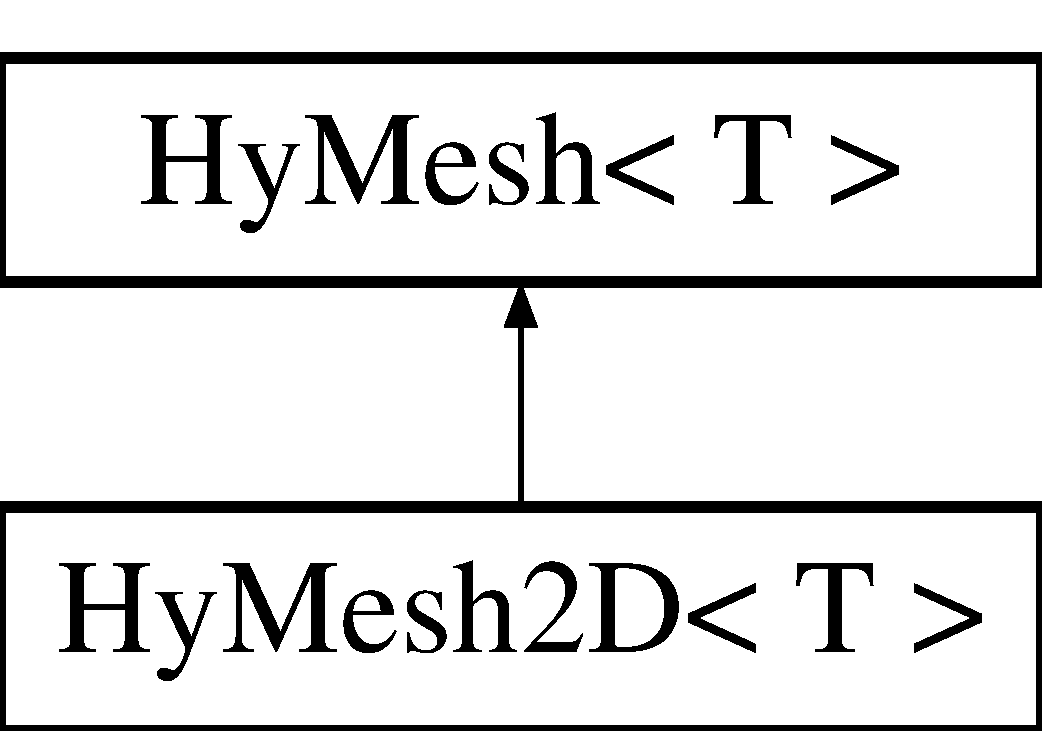
\includegraphics[height=2cm]{classHyMesh2D}
\end{center}
\end{figure}
\subsection*{Public Member Functions}
\begin{DoxyCompactItemize}
\item 
\hypertarget{classHyMesh2D_ad6cb9da096558be08d3fa3c1f8929410}{
\hyperlink{classHyMesh2D_ad6cb9da096558be08d3fa3c1f8929410}{HyMesh2D} ()}
\label{classHyMesh2D_ad6cb9da096558be08d3fa3c1f8929410}

\begin{DoxyCompactList}\small\item\em Default constructor. \item\end{DoxyCompactList}\item 
\hyperlink{classHyMesh2D_a0b73e736d5f0a2fc253d4ef724968b1f}{HyMesh2D} (\hyperlink{classHyPoint}{HyPoint}$<$ T $>$ \&pBL, \hyperlink{classHyPoint}{HyPoint}$<$ T $>$ \&pUR, unsigned long pNbRectanglesX, unsigned long pNbRectanglesY)
\begin{DoxyCompactList}\small\item\em Constructor. \item\end{DoxyCompactList}\item 
\hyperlink{classHyMesh2D_addcbe5c16210083bf69b1210ea11d569}{HyMesh2D} (\hyperlink{classHyMesh2D}{HyMesh2D}$<$ T $>$ \&pMesh)
\begin{DoxyCompactList}\small\item\em Copy constructor. \item\end{DoxyCompactList}\item 
std::vector$<$ std::vector$<$ \hyperlink{classHyPoint}{HyPoint}$<$ T $>$ $>$ $>$ \& \hyperlink{classHyMesh2D_a8f075d7ba59bc759dc138109fd551496}{getMesh} ()
\begin{DoxyCompactList}\small\item\em Getter to aMesh attribute. \item\end{DoxyCompactList}\item 
unsigned long \hyperlink{classHyMesh2D_a8646d6b9e0b42270744a2b3c15af2563}{getNbRectanglesX} ()
\begin{DoxyCompactList}\small\item\em Getter to aNbRectanglesX attribute. \item\end{DoxyCompactList}\item 
unsigned long \hyperlink{classHyMesh2D_af247c2440a04397980270bb0b4410225}{getNbRectanglesY} ()
\begin{DoxyCompactList}\small\item\em Getter to aNbRectanglesY attribute. \item\end{DoxyCompactList}\item 
double \hyperlink{classHyMesh2D_aa3c7f4d72c521783c2b358b6f7b73031}{getHX} ()
\begin{DoxyCompactList}\small\item\em Getter to ahX attribute. \item\end{DoxyCompactList}\item 
double \hyperlink{classHyMesh2D_a94d54a398cb5d0de0b083b03926d698e}{getHY} ()
\begin{DoxyCompactList}\small\item\em Getter to ahY attribute. \item\end{DoxyCompactList}\item 
unsigned long \hyperlink{classHyMesh2D_a109323e7c482899df86c76102ff3a5e8}{size} ()
\begin{DoxyCompactList}\small\item\em Number of points in the mesh. \item\end{DoxyCompactList}\item 
\hypertarget{classHyMesh2D_ae2cb45f669fcbb6e340488efc8811d94}{
std::vector$<$ \hyperlink{classHyPoint}{HyPoint}$<$ T $>$ $>$ \& \hyperlink{classHyMesh2D_ae2cb45f669fcbb6e340488efc8811d94}{operator\mbox{[}$\,$\mbox{]}} (unsigned long i)}
\label{classHyMesh2D_ae2cb45f669fcbb6e340488efc8811d94}

\begin{DoxyCompactList}\small\item\em operator\mbox{[}\mbox{]} \item\end{DoxyCompactList}\item 
\hypertarget{classHyMesh2D_a39651f07d9d3d8afc6b6f80b7883df71}{
void {\bfseries display} ()}
\label{classHyMesh2D_a39651f07d9d3d8afc6b6f80b7883df71}

\end{DoxyCompactItemize}
\subsection*{Protected Attributes}
\begin{DoxyCompactItemize}
\item 
std::vector$<$ std::vector$<$ \hyperlink{classHyPoint}{HyPoint}$<$ T $>$ $>$ $>$ \hyperlink{classHyMesh2D_af82a94a4943d2da5637d0bbc0b405eed}{aMesh}
\item 
unsigned long \hyperlink{classHyMesh2D_a53430a7d9168ad8e9392252b87e139eb}{aNbRectanglesX}
\item 
unsigned long \hyperlink{classHyMesh2D_a836a8033b37ffdb7103510eabb1b3055}{aNbRectanglesY}
\item 
double \hyperlink{classHyMesh2D_a613e4597dc45ca5629ec46eb941e9db8}{ahX}
\item 
double \hyperlink{classHyMesh2D_a90e7b6ebe92fca8ad22795899ec8500b}{ahY}
\end{DoxyCompactItemize}


\subsection{Detailed Description}
\subsubsection*{template$<$typename T$>$ class HyMesh2D$<$ T $>$}

Two dimensional mesh. 

\subsection{Constructor \& Destructor Documentation}
\hypertarget{classHyMesh2D_a0b73e736d5f0a2fc253d4ef724968b1f}{
\index{HyMesh2D@{HyMesh2D}!HyMesh2D@{HyMesh2D}}
\index{HyMesh2D@{HyMesh2D}!HyMesh2D@{HyMesh2D}}
\subsubsection[{HyMesh2D}]{\setlength{\rightskip}{0pt plus 5cm}template$<$typename T $>$ {\bf HyMesh2D}$<$ T $>$::{\bf HyMesh2D} ({\bf HyPoint}$<$ T $>$ \& {\em pBL}, \/  {\bf HyPoint}$<$ T $>$ \& {\em pUR}, \/  unsigned long {\em pNbRectanglesX}, \/  unsigned long {\em pNbRectanglesY})\hspace{0.3cm}{\ttfamily  \mbox{[}inline\mbox{]}}}}
\label{classHyMesh2D_a0b73e736d5f0a2fc253d4ef724968b1f}


Constructor. 


\begin{DoxyParams}{Parameters}
\item[{\em pBL}]: The Bottom Left point \item[{\em pUR}]: The Upper Right point \item[{\em pNbRectanglesX}]: Number of nodes on X-\/axis \item[{\em pNbRectanglesY}]: Number of nodes on Y-\/axis \end{DoxyParams}
\hypertarget{classHyMesh2D_addcbe5c16210083bf69b1210ea11d569}{
\index{HyMesh2D@{HyMesh2D}!HyMesh2D@{HyMesh2D}}
\index{HyMesh2D@{HyMesh2D}!HyMesh2D@{HyMesh2D}}
\subsubsection[{HyMesh2D}]{\setlength{\rightskip}{0pt plus 5cm}template$<$typename T $>$ {\bf HyMesh2D}$<$ T $>$::{\bf HyMesh2D} ({\bf HyMesh2D}$<$ T $>$ \& {\em pMesh})\hspace{0.3cm}{\ttfamily  \mbox{[}inline\mbox{]}}}}
\label{classHyMesh2D_addcbe5c16210083bf69b1210ea11d569}


Copy constructor. 


\begin{DoxyParams}{Parameters}
\item[{\em pMesh}]: Reference to another \hyperlink{classHyMesh}{HyMesh} \end{DoxyParams}


\subsection{Member Function Documentation}
\hypertarget{classHyMesh2D_aa3c7f4d72c521783c2b358b6f7b73031}{
\index{HyMesh2D@{HyMesh2D}!getHX@{getHX}}
\index{getHX@{getHX}!HyMesh2D@{HyMesh2D}}
\subsubsection[{getHX}]{\setlength{\rightskip}{0pt plus 5cm}template$<$typename T$>$ double {\bf HyMesh2D}$<$ T $>$::getHX ()\hspace{0.3cm}{\ttfamily  \mbox{[}inline\mbox{]}}}}
\label{classHyMesh2D_aa3c7f4d72c521783c2b358b6f7b73031}


Getter to ahX attribute. 

\begin{DoxyReturn}{Returns}
ahX 
\end{DoxyReturn}
\hypertarget{classHyMesh2D_a94d54a398cb5d0de0b083b03926d698e}{
\index{HyMesh2D@{HyMesh2D}!getHY@{getHY}}
\index{getHY@{getHY}!HyMesh2D@{HyMesh2D}}
\subsubsection[{getHY}]{\setlength{\rightskip}{0pt plus 5cm}template$<$typename T$>$ double {\bf HyMesh2D}$<$ T $>$::getHY ()\hspace{0.3cm}{\ttfamily  \mbox{[}inline\mbox{]}}}}
\label{classHyMesh2D_a94d54a398cb5d0de0b083b03926d698e}


Getter to ahY attribute. 

\begin{DoxyReturn}{Returns}
ahY 
\end{DoxyReturn}
\hypertarget{classHyMesh2D_a8f075d7ba59bc759dc138109fd551496}{
\index{HyMesh2D@{HyMesh2D}!getMesh@{getMesh}}
\index{getMesh@{getMesh}!HyMesh2D@{HyMesh2D}}
\subsubsection[{getMesh}]{\setlength{\rightskip}{0pt plus 5cm}template$<$typename T$>$ std::vector$<$ std::vector$<$ {\bf HyPoint}$<$T$>$ $>$ $>$\& {\bf HyMesh2D}$<$ T $>$::getMesh ()\hspace{0.3cm}{\ttfamily  \mbox{[}inline\mbox{]}}}}
\label{classHyMesh2D_a8f075d7ba59bc759dc138109fd551496}


Getter to aMesh attribute. 

\begin{DoxyReturn}{Returns}
Reference to aMesh 
\end{DoxyReturn}
\hypertarget{classHyMesh2D_a8646d6b9e0b42270744a2b3c15af2563}{
\index{HyMesh2D@{HyMesh2D}!getNbRectanglesX@{getNbRectanglesX}}
\index{getNbRectanglesX@{getNbRectanglesX}!HyMesh2D@{HyMesh2D}}
\subsubsection[{getNbRectanglesX}]{\setlength{\rightskip}{0pt plus 5cm}template$<$typename T$>$ unsigned long {\bf HyMesh2D}$<$ T $>$::getNbRectanglesX ()\hspace{0.3cm}{\ttfamily  \mbox{[}inline\mbox{]}}}}
\label{classHyMesh2D_a8646d6b9e0b42270744a2b3c15af2563}


Getter to aNbRectanglesX attribute. 

\begin{DoxyReturn}{Returns}
aNbRectanglesX 
\end{DoxyReturn}
\hypertarget{classHyMesh2D_af247c2440a04397980270bb0b4410225}{
\index{HyMesh2D@{HyMesh2D}!getNbRectanglesY@{getNbRectanglesY}}
\index{getNbRectanglesY@{getNbRectanglesY}!HyMesh2D@{HyMesh2D}}
\subsubsection[{getNbRectanglesY}]{\setlength{\rightskip}{0pt plus 5cm}template$<$typename T$>$ unsigned long {\bf HyMesh2D}$<$ T $>$::getNbRectanglesY ()\hspace{0.3cm}{\ttfamily  \mbox{[}inline\mbox{]}}}}
\label{classHyMesh2D_af247c2440a04397980270bb0b4410225}


Getter to aNbRectanglesY attribute. 

\begin{DoxyReturn}{Returns}
aNbRectanglesY 
\end{DoxyReturn}
\hypertarget{classHyMesh2D_a109323e7c482899df86c76102ff3a5e8}{
\index{HyMesh2D@{HyMesh2D}!size@{size}}
\index{size@{size}!HyMesh2D@{HyMesh2D}}
\subsubsection[{size}]{\setlength{\rightskip}{0pt plus 5cm}template$<$typename T$>$ unsigned long {\bf HyMesh2D}$<$ T $>$::size ()\hspace{0.3cm}{\ttfamily  \mbox{[}inline\mbox{]}}}}
\label{classHyMesh2D_a109323e7c482899df86c76102ff3a5e8}


Number of points in the mesh. 

\begin{DoxyReturn}{Returns}
The number of points in the mesh 
\end{DoxyReturn}


\subsection{Member Data Documentation}
\hypertarget{classHyMesh2D_a613e4597dc45ca5629ec46eb941e9db8}{
\index{HyMesh2D@{HyMesh2D}!ahX@{ahX}}
\index{ahX@{ahX}!HyMesh2D@{HyMesh2D}}
\subsubsection[{ahX}]{\setlength{\rightskip}{0pt plus 5cm}template$<$typename T$>$ double {\bf HyMesh2D}$<$ T $>$::{\bf ahX}\hspace{0.3cm}{\ttfamily  \mbox{[}protected\mbox{]}}}}
\label{classHyMesh2D_a613e4597dc45ca5629ec46eb941e9db8}
Size between two nodes on X-\/axis \hypertarget{classHyMesh2D_a90e7b6ebe92fca8ad22795899ec8500b}{
\index{HyMesh2D@{HyMesh2D}!ahY@{ahY}}
\index{ahY@{ahY}!HyMesh2D@{HyMesh2D}}
\subsubsection[{ahY}]{\setlength{\rightskip}{0pt plus 5cm}template$<$typename T$>$ double {\bf HyMesh2D}$<$ T $>$::{\bf ahY}\hspace{0.3cm}{\ttfamily  \mbox{[}protected\mbox{]}}}}
\label{classHyMesh2D_a90e7b6ebe92fca8ad22795899ec8500b}
Size between two nodes on Y-\/axis \hypertarget{classHyMesh2D_af82a94a4943d2da5637d0bbc0b405eed}{
\index{HyMesh2D@{HyMesh2D}!aMesh@{aMesh}}
\index{aMesh@{aMesh}!HyMesh2D@{HyMesh2D}}
\subsubsection[{aMesh}]{\setlength{\rightskip}{0pt plus 5cm}template$<$typename T$>$ std::vector$<$ std::vector$<${\bf HyPoint}$<$T$>$ $>$ $>$ {\bf HyMesh2D}$<$ T $>$::{\bf aMesh}\hspace{0.3cm}{\ttfamily  \mbox{[}protected\mbox{]}}}}
\label{classHyMesh2D_af82a94a4943d2da5637d0bbc0b405eed}
The mesh \hypertarget{classHyMesh2D_a53430a7d9168ad8e9392252b87e139eb}{
\index{HyMesh2D@{HyMesh2D}!aNbRectanglesX@{aNbRectanglesX}}
\index{aNbRectanglesX@{aNbRectanglesX}!HyMesh2D@{HyMesh2D}}
\subsubsection[{aNbRectanglesX}]{\setlength{\rightskip}{0pt plus 5cm}template$<$typename T$>$ unsigned long {\bf HyMesh2D}$<$ T $>$::{\bf aNbRectanglesX}\hspace{0.3cm}{\ttfamily  \mbox{[}protected\mbox{]}}}}
\label{classHyMesh2D_a53430a7d9168ad8e9392252b87e139eb}
Number of nodes on X-\/axis \hypertarget{classHyMesh2D_a836a8033b37ffdb7103510eabb1b3055}{
\index{HyMesh2D@{HyMesh2D}!aNbRectanglesY@{aNbRectanglesY}}
\index{aNbRectanglesY@{aNbRectanglesY}!HyMesh2D@{HyMesh2D}}
\subsubsection[{aNbRectanglesY}]{\setlength{\rightskip}{0pt plus 5cm}template$<$typename T$>$ unsigned long {\bf HyMesh2D}$<$ T $>$::{\bf aNbRectanglesY}\hspace{0.3cm}{\ttfamily  \mbox{[}protected\mbox{]}}}}
\label{classHyMesh2D_a836a8033b37ffdb7103510eabb1b3055}
Number of nodes on Y-\/axis 

The documentation for this class was generated from the following files:\begin{DoxyCompactItemize}
\item 
\hyperlink{HyMesh2D_8hpp}{HyMesh2D.hpp}\item 
HyMesh2D.ipp\end{DoxyCompactItemize}

\hypertarget{classHyPlotter}{
\section{HyPlotter$<$ T $>$ Class Template Reference}
\label{classHyPlotter}\index{HyPlotter@{HyPlotter}}
}


This class is used for post-\/processing analysis. Given a \hyperlink{classHyMesh}{HyMesh} and a set of data, it saves the solution in a file.  




{\ttfamily \#include $<$HyPlotter.hpp$>$}

\subsection*{Public Member Functions}
\begin{DoxyCompactItemize}
\item 
\hypertarget{classHyPlotter_a50b452f5b5747d4505e2e9e85943fbd1}{
\hyperlink{classHyPlotter_a50b452f5b5747d4505e2e9e85943fbd1}{HyPlotter} ()}
\label{classHyPlotter_a50b452f5b5747d4505e2e9e85943fbd1}

\begin{DoxyCompactList}\small\item\em Default constructor of \hyperlink{classHyPlotter}{HyPlotter}. \item\end{DoxyCompactList}\item 
\hypertarget{classHyPlotter_ace9cd6b9ea3082dc8e31f5b6461deb6b}{
{\bfseries HyPlotter} (\hyperlink{classHyMesh2D}{HyMesh2D}$<$ T $>$ pMesh, std::vector$<$ Eigen::VectorXd $>$ pData, std::string pFileName)}
\label{classHyPlotter_ace9cd6b9ea3082dc8e31f5b6461deb6b}

\item 
std::string \hyperlink{classHyPlotter_a3901644f0e38b620ebe2c02b2198aa23}{intToString} (unsigned long int n)
\begin{DoxyCompactList}\small\item\em Converts an integer to a string. \item\end{DoxyCompactList}\item 
void \hyperlink{classHyPlotter_acb107c1c3cf44bb32b900c329830fdfd}{save} (std::string pFolder)
\begin{DoxyCompactList}\small\item\em Save the data in files. In case of a time dependent solution (several VectorXd), suffixes will be written for the name of the files. \item\end{DoxyCompactList}\end{DoxyCompactItemize}
\subsection*{Protected Attributes}
\begin{DoxyCompactItemize}
\item 
\hyperlink{classHyMesh2D}{HyMesh2D}$<$ T $>$ \hyperlink{classHyPlotter_add8bc0e65fe86f1e8efb025afd679f70}{aMesh}
\item 
std::vector$<$ Eigen::VectorXd $>$ \hyperlink{classHyPlotter_a9aa282a34786a8d215a28b43816a2e6c}{aData}
\item 
std::string \hyperlink{classHyPlotter_a7ff236b2b02b1ee33554d0c2d483ca83}{aFileName}
\end{DoxyCompactItemize}


\subsection{Detailed Description}
\subsubsection*{template$<$typename T$>$ class HyPlotter$<$ T $>$}

This class is used for post-\/processing analysis. Given a \hyperlink{classHyMesh}{HyMesh} and a set of data, it saves the solution in a file. 

\subsection{Member Function Documentation}
\hypertarget{classHyPlotter_a3901644f0e38b620ebe2c02b2198aa23}{
\index{HyPlotter@{HyPlotter}!intToString@{intToString}}
\index{intToString@{intToString}!HyPlotter@{HyPlotter}}
\subsubsection[{intToString}]{\setlength{\rightskip}{0pt plus 5cm}template$<$typename T $>$ std::string {\bf HyPlotter}$<$ T $>$::intToString (unsigned long int {\em n})\hspace{0.3cm}{\ttfamily  \mbox{[}inline\mbox{]}}}}
\label{classHyPlotter_a3901644f0e38b620ebe2c02b2198aa23}


Converts an integer to a string. 


\begin{DoxyParams}{Parameters}
\item[{\em n}]The integer to convert to string. \end{DoxyParams}
\hypertarget{classHyPlotter_acb107c1c3cf44bb32b900c329830fdfd}{
\index{HyPlotter@{HyPlotter}!save@{save}}
\index{save@{save}!HyPlotter@{HyPlotter}}
\subsubsection[{save}]{\setlength{\rightskip}{0pt plus 5cm}template$<$typename T $>$ void {\bf HyPlotter}$<$ T $>$::save (std::string {\em pFolder})\hspace{0.3cm}{\ttfamily  \mbox{[}inline\mbox{]}}}}
\label{classHyPlotter_acb107c1c3cf44bb32b900c329830fdfd}


Save the data in files. In case of a time dependent solution (several VectorXd), suffixes will be written for the name of the files. 


\begin{DoxyParams}{Parameters}
\item[{\em pFolder}]The folder to save files in. \end{DoxyParams}


\subsection{Member Data Documentation}
\hypertarget{classHyPlotter_a9aa282a34786a8d215a28b43816a2e6c}{
\index{HyPlotter@{HyPlotter}!aData@{aData}}
\index{aData@{aData}!HyPlotter@{HyPlotter}}
\subsubsection[{aData}]{\setlength{\rightskip}{0pt plus 5cm}template$<$typename T $>$ std::vector$<$Eigen::VectorXd$>$ {\bf HyPlotter}$<$ T $>$::{\bf aData}\hspace{0.3cm}{\ttfamily  \mbox{[}protected\mbox{]}}}}
\label{classHyPlotter_a9aa282a34786a8d215a28b43816a2e6c}
The values corresponding to each point of the mesh \hypertarget{classHyPlotter_a7ff236b2b02b1ee33554d0c2d483ca83}{
\index{HyPlotter@{HyPlotter}!aFileName@{aFileName}}
\index{aFileName@{aFileName}!HyPlotter@{HyPlotter}}
\subsubsection[{aFileName}]{\setlength{\rightskip}{0pt plus 5cm}template$<$typename T $>$ std::string {\bf HyPlotter}$<$ T $>$::{\bf aFileName}\hspace{0.3cm}{\ttfamily  \mbox{[}protected\mbox{]}}}}
\label{classHyPlotter_a7ff236b2b02b1ee33554d0c2d483ca83}
The name of the file to save in \hypertarget{classHyPlotter_add8bc0e65fe86f1e8efb025afd679f70}{
\index{HyPlotter@{HyPlotter}!aMesh@{aMesh}}
\index{aMesh@{aMesh}!HyPlotter@{HyPlotter}}
\subsubsection[{aMesh}]{\setlength{\rightskip}{0pt plus 5cm}template$<$typename T $>$ {\bf HyMesh2D}$<$T$>$ {\bf HyPlotter}$<$ T $>$::{\bf aMesh}\hspace{0.3cm}{\ttfamily  \mbox{[}protected\mbox{]}}}}
\label{classHyPlotter_add8bc0e65fe86f1e8efb025afd679f70}
The mesh 

The documentation for this class was generated from the following files:\begin{DoxyCompactItemize}
\item 
\hyperlink{HyPlotter_8hpp}{HyPlotter.hpp}\item 
\hyperlink{HyPlotter_8ipp}{HyPlotter.ipp}\end{DoxyCompactItemize}

\hypertarget{classHyPoint}{
\section{HyPoint$<$ T $>$ Class Template Reference}
\label{classHyPoint}\index{HyPoint@{HyPoint}}
}
\subsection*{Public Member Functions}
\begin{DoxyCompactItemize}
\item 
\hypertarget{classHyPoint_a7a2e22bc7a8dca02d24a2d912ca6f9b5}{
{\bfseries HyPoint} (T pX, T pY, T pZ, unsigned long pID, bool pRegular)}
\label{classHyPoint_a7a2e22bc7a8dca02d24a2d912ca6f9b5}

\item 
\hypertarget{classHyPoint_ad7001ba0937ec5dfb2ed24971a1010c3}{
{\bfseries HyPoint} (const \hyperlink{classHyPoint}{HyPoint}$<$ T $>$ \&pP)}
\label{classHyPoint_ad7001ba0937ec5dfb2ed24971a1010c3}

\item 
\hypertarget{classHyPoint_a93b8eec7ce456bec263dc58c4f874909}{
T {\bfseries getX} () const }
\label{classHyPoint_a93b8eec7ce456bec263dc58c4f874909}

\item 
\hypertarget{classHyPoint_ae2e111bf01c6df94a288b7dd6c9eeb47}{
T {\bfseries getY} () const }
\label{classHyPoint_ae2e111bf01c6df94a288b7dd6c9eeb47}

\item 
\hypertarget{classHyPoint_a08f9cf8a0e917427e034208bb6329e11}{
T {\bfseries getZ} () const }
\label{classHyPoint_a08f9cf8a0e917427e034208bb6329e11}

\item 
\hypertarget{classHyPoint_ad4d4bd3a4d53f31431b530728e84aa16}{
unsigned long {\bfseries getID} () const }
\label{classHyPoint_ad4d4bd3a4d53f31431b530728e84aa16}

\item 
\hypertarget{classHyPoint_a69b5f761ddd90503dbea866ffdb33405}{
bool {\bfseries getRegularity} () const }
\label{classHyPoint_a69b5f761ddd90503dbea866ffdb33405}

\item 
\hypertarget{classHyPoint_a65d48c97d8bdfdcbdb24338470117ab7}{
int {\bfseries getLocality} () const }
\label{classHyPoint_a65d48c97d8bdfdcbdb24338470117ab7}

\item 
\hypertarget{classHyPoint_a9ca2e309a2b8f23f84f655fa18699c8d}{
\hyperlink{classHyPoint}{HyPoint} $\ast$ {\bfseries getNeigW} () const }
\label{classHyPoint_a9ca2e309a2b8f23f84f655fa18699c8d}

\item 
\hypertarget{classHyPoint_a4ed40cda2b5cfd3b41b6086af7410672}{
\hyperlink{classHyPoint}{HyPoint} $\ast$ {\bfseries getNeigE} () const }
\label{classHyPoint_a4ed40cda2b5cfd3b41b6086af7410672}

\item 
\hypertarget{classHyPoint_a065d40f1b4b39ec6fe1ed08d091aa6c4}{
\hyperlink{classHyPoint}{HyPoint} $\ast$ {\bfseries getNeigN} () const }
\label{classHyPoint_a065d40f1b4b39ec6fe1ed08d091aa6c4}

\item 
\hypertarget{classHyPoint_aed6b8820c2fc550dabe218226a5c6b3a}{
\hyperlink{classHyPoint}{HyPoint} $\ast$ {\bfseries getNeigS} () const }
\label{classHyPoint_aed6b8820c2fc550dabe218226a5c6b3a}

\item 
\hypertarget{classHyPoint_a94d4e7e10944470b74126f1c3a6a2f01}{
bool {\bfseries getBoundary} () const }
\label{classHyPoint_a94d4e7e10944470b74126f1c3a6a2f01}

\item 
\hypertarget{classHyPoint_a4018195efa41a7afcdd30ba31328f40d}{
void {\bfseries setX} (T pX)}
\label{classHyPoint_a4018195efa41a7afcdd30ba31328f40d}

\item 
\hypertarget{classHyPoint_ae4b88fe2a4891bfed3f89b8b3b6cb5ee}{
void {\bfseries setY} (T pY)}
\label{classHyPoint_ae4b88fe2a4891bfed3f89b8b3b6cb5ee}

\item 
\hypertarget{classHyPoint_a254f134830768f320553de91e86c410e}{
void {\bfseries setZ} (T pZ)}
\label{classHyPoint_a254f134830768f320553de91e86c410e}

\item 
\hypertarget{classHyPoint_a5419bc2b6020d99fe0481527b4c4ba26}{
void {\bfseries setID} (unsigned long int pID)}
\label{classHyPoint_a5419bc2b6020d99fe0481527b4c4ba26}

\item 
\hypertarget{classHyPoint_a4697b7c1d639b05e65a55c3f198fe1a5}{
void {\bfseries setRegularity} (bool pRegular)}
\label{classHyPoint_a4697b7c1d639b05e65a55c3f198fe1a5}

\item 
\hypertarget{classHyPoint_acbea140c1fbb8ac056d71df4ce502e60}{
void {\bfseries setLocality} (int pLocality)}
\label{classHyPoint_acbea140c1fbb8ac056d71df4ce502e60}

\item 
\hypertarget{classHyPoint_aede484eae10b7fa0ca5345b4bd75f824}{
void {\bfseries setNeigW} (\hyperlink{classHyPoint}{HyPoint} $\ast$pNeig)}
\label{classHyPoint_aede484eae10b7fa0ca5345b4bd75f824}

\item 
\hypertarget{classHyPoint_acaacdb655b793db593a7ffd968fe8ea4}{
void {\bfseries setNeigE} (\hyperlink{classHyPoint}{HyPoint} $\ast$pNeig)}
\label{classHyPoint_acaacdb655b793db593a7ffd968fe8ea4}

\item 
\hypertarget{classHyPoint_a851718a6acc6e5256bad58197a3821b3}{
void {\bfseries setNeigN} (\hyperlink{classHyPoint}{HyPoint} $\ast$pNeig)}
\label{classHyPoint_a851718a6acc6e5256bad58197a3821b3}

\item 
\hypertarget{classHyPoint_ad3118592f2de1c104ebd9c0e417f59d5}{
void {\bfseries setNeigS} (\hyperlink{classHyPoint}{HyPoint} $\ast$pNeig)}
\label{classHyPoint_ad3118592f2de1c104ebd9c0e417f59d5}

\item 
\hypertarget{classHyPoint_ab397f4700d45568e1e1bd07010d35704}{
void {\bfseries setBoundary} (bool pBoundary)}
\label{classHyPoint_ab397f4700d45568e1e1bd07010d35704}

\item 
\hypertarget{classHyPoint_adec1f5535f3b40fa16980969df05b87c}{
\hyperlink{classHyPoint}{HyPoint}$<$ T $>$ \& {\bfseries operator=} (const \hyperlink{classHyPoint}{HyPoint}$<$ T $>$ \&pPoint)}
\label{classHyPoint_adec1f5535f3b40fa16980969df05b87c}

\item 
\hypertarget{classHyPoint_aa7f50007090adfd1733276951cb05983}{
bool {\bfseries operator==} (const \hyperlink{classHyPoint}{HyPoint}$<$ T $>$ \&pPoint)}
\label{classHyPoint_aa7f50007090adfd1733276951cb05983}

\item 
\hypertarget{classHyPoint_ad7adaa5c49d54fe6ba0dbb9024a9c6eb}{
bool {\bfseries operator!=} (const \hyperlink{classHyPoint}{HyPoint}$<$ T $>$ \&pPoint)}
\label{classHyPoint_ad7adaa5c49d54fe6ba0dbb9024a9c6eb}

\item 
\hypertarget{classHyPoint_a5be21cb2e4a3e1d3779247c2391e1f07}{
double {\bfseries distance} (const \hyperlink{classHyPoint}{HyPoint}$<$ T $>$ \&pPoint)}
\label{classHyPoint_a5be21cb2e4a3e1d3779247c2391e1f07}

\item 
\hypertarget{classHyPoint_ac18ecf354862fb870aa3957c94c22eb9}{
double {\bfseries sqDistance} (const \hyperlink{classHyPoint}{HyPoint}$<$ T $>$ \&pPoint)}
\label{classHyPoint_ac18ecf354862fb870aa3957c94c22eb9}

\end{DoxyCompactItemize}
\subsection*{Protected Attributes}
\begin{DoxyCompactItemize}
\item 
\hypertarget{classHyPoint_a621a7b4dc8f10a4b3b3ba6889984f679}{
T {\bfseries aX}}
\label{classHyPoint_a621a7b4dc8f10a4b3b3ba6889984f679}

\item 
\hypertarget{classHyPoint_ad73bb2928402cf7b742f4112bf0ab027}{
T {\bfseries aY}}
\label{classHyPoint_ad73bb2928402cf7b742f4112bf0ab027}

\item 
\hypertarget{classHyPoint_a556c7c43914d1142d323a261e9b80991}{
T {\bfseries aZ}}
\label{classHyPoint_a556c7c43914d1142d323a261e9b80991}

\item 
\hypertarget{classHyPoint_a03b4fa88c8d1e26d334db8708c3e1ade}{
unsigned long {\bfseries aID}}
\label{classHyPoint_a03b4fa88c8d1e26d334db8708c3e1ade}

\item 
\hypertarget{classHyPoint_a970648d0e335272cb70496890d34f3d4}{
bool {\bfseries aRegular}}
\label{classHyPoint_a970648d0e335272cb70496890d34f3d4}

\item 
\hypertarget{classHyPoint_a0e40b31ce4bdea3dd2eb450245a532ae}{
int {\bfseries aLocality}}
\label{classHyPoint_a0e40b31ce4bdea3dd2eb450245a532ae}

\item 
\hypertarget{classHyPoint_aa7692363efc10f709cb7df258b8c1dde}{
\hyperlink{classHyPoint}{HyPoint} $\ast$ {\bfseries aNeigW}}
\label{classHyPoint_aa7692363efc10f709cb7df258b8c1dde}

\item 
\hypertarget{classHyPoint_ae4718bd52b919a1bff3496450ccc62ad}{
\hyperlink{classHyPoint}{HyPoint} $\ast$ {\bfseries aNeigE}}
\label{classHyPoint_ae4718bd52b919a1bff3496450ccc62ad}

\item 
\hypertarget{classHyPoint_a7e3d2c15bdace44908252b79be164925}{
\hyperlink{classHyPoint}{HyPoint} $\ast$ {\bfseries aNeigN}}
\label{classHyPoint_a7e3d2c15bdace44908252b79be164925}

\item 
\hypertarget{classHyPoint_a47aa9914ea1a270a4c8a74ca0f89a5b8}{
\hyperlink{classHyPoint}{HyPoint} $\ast$ {\bfseries aNeigS}}
\label{classHyPoint_a47aa9914ea1a270a4c8a74ca0f89a5b8}

\item 
\hypertarget{classHyPoint_adc04d93e4200154433e0bace08df3e8a}{
bool {\bfseries aBoundary}}
\label{classHyPoint_adc04d93e4200154433e0bace08df3e8a}

\end{DoxyCompactItemize}
\subsubsection*{template$<$typename T$>$ class HyPoint$<$ T $>$}



The documentation for this class was generated from the following files:\begin{DoxyCompactItemize}
\item 
\hyperlink{HyPoint_8hpp}{HyPoint.hpp}\item 
HyPoint.ipp\end{DoxyCompactItemize}

\hypertarget{classHyPoisson2D}{
\section{HyPoisson2D$<$ T $>$ Class Template Reference}
\label{classHyPoisson2D}\index{HyPoisson2D@{HyPoisson2D}}
}


Poisson equation in 2 dimensions: $ \Delta u = f $.  




{\ttfamily \#include $<$HyPoisson2D.hpp$>$}

Inheritance diagram for HyPoisson2D$<$ T $>$:\begin{figure}[H]
\begin{center}
\leavevmode
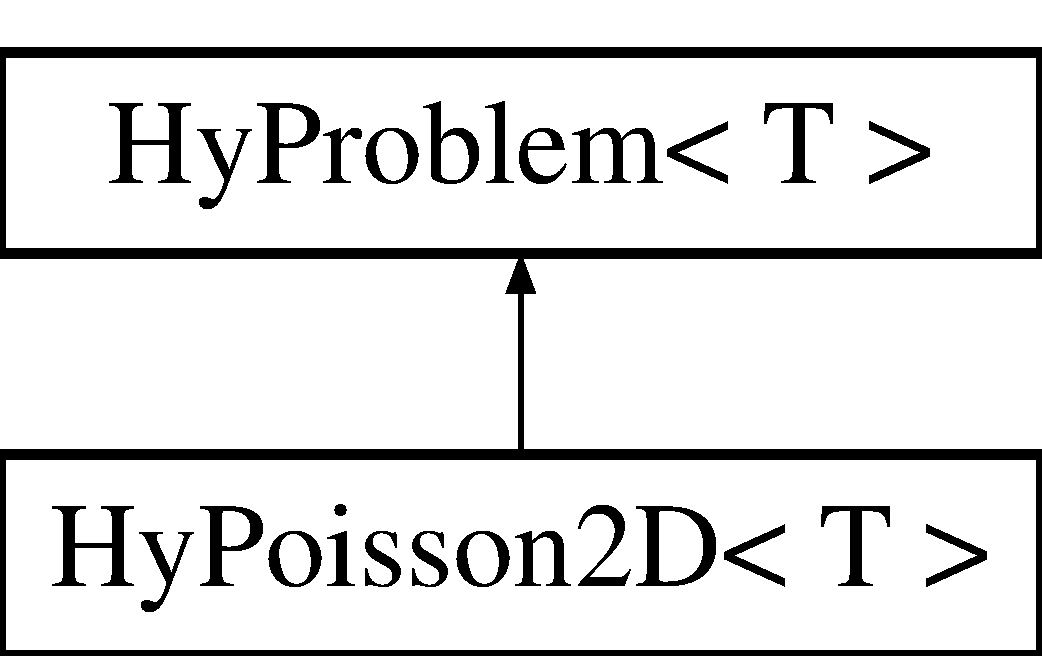
\includegraphics[height=2cm]{classHyPoisson2D}
\end{center}
\end{figure}
\subsection*{Public Member Functions}
\begin{DoxyCompactItemize}
\item 
\hypertarget{classHyPoisson2D_a1ce5db0977faea87271b5c48c89121bc}{
\hyperlink{classHyPoisson2D_a1ce5db0977faea87271b5c48c89121bc}{HyPoisson2D} ()}
\label{classHyPoisson2D_a1ce5db0977faea87271b5c48c89121bc}

\begin{DoxyCompactList}\small\item\em Default constructor. \item\end{DoxyCompactList}\item 
\hypertarget{classHyPoisson2D_a090399fc99e38625d92397aae07d5732}{
{\bfseries HyPoisson2D} (\hyperlink{classHyDomain}{HyDomain}$<$ T $>$ \&pDomain, \hyperlink{classHyBoundary}{HyBoundary}$<$ T $>$ \&pBoundary, \hyperlink{classHyMesh2D}{HyMesh2D}$<$ T $>$ \&pMesh, std::string \&pDescription)}
\label{classHyPoisson2D_a090399fc99e38625d92397aae07d5732}

\item 
\hypertarget{classHyPoisson2D_a4b5fa83627d8a1ec9716888d69217034}{
void \hyperlink{classHyPoisson2D_a4b5fa83627d8a1ec9716888d69217034}{build} ()}
\label{classHyPoisson2D_a4b5fa83627d8a1ec9716888d69217034}

\begin{DoxyCompactList}\small\item\em Fills the matrix A and the vectors F and G. \item\end{DoxyCompactList}\item 
\hypertarget{classHyPoisson2D_a905070be03612344705d81e72759ba32}{
void {\bfseries solve} ()}
\label{classHyPoisson2D_a905070be03612344705d81e72759ba32}

\item 
double \hyperlink{classHyPoisson2D_a9c27e90e3abb3a6ebe5d6b3274412e7a}{g} (\hyperlink{classHyPoint}{HyPoint}$<$ T $>$ pPoint)
\begin{DoxyCompactList}\small\item\em The Dirichlet condition on the boundary. \item\end{DoxyCompactList}\item 
\hypertarget{classHyPoisson2D_a26b5243fcf822a4009abeb72fb8cb01d}{
double {\bfseries g} (T pX, T pY, T pZ)}
\label{classHyPoisson2D_a26b5243fcf822a4009abeb72fb8cb01d}

\item 
double \hyperlink{classHyPoisson2D_ace05fcef4dbe0fe29c1357f7b0eeed23}{f} (\hyperlink{classHyPoint}{HyPoint}$<$ T $>$ pPoint)
\begin{DoxyCompactList}\small\item\em The function f. \item\end{DoxyCompactList}\item 
double \hyperlink{classHyPoisson2D_a8d4e172777a6adaa792d61f86b480e08}{f} (T pX, T pY)
\begin{DoxyCompactList}\small\item\em The function f. \item\end{DoxyCompactList}\end{DoxyCompactItemize}


\subsection{Detailed Description}
\subsubsection*{template$<$typename T$>$ class HyPoisson2D$<$ T $>$}

Poisson equation in 2 dimensions: $ \Delta u = f $. 

\subsection{Member Function Documentation}
\hypertarget{classHyPoisson2D_a8d4e172777a6adaa792d61f86b480e08}{
\index{HyPoisson2D@{HyPoisson2D}!f@{f}}
\index{f@{f}!HyPoisson2D@{HyPoisson2D}}
\subsubsection[{f}]{\setlength{\rightskip}{0pt plus 5cm}template$<$typename T $>$ double {\bf HyPoisson2D}$<$ T $>$::f (T {\em pX}, \/  T {\em pY})\hspace{0.3cm}{\ttfamily  \mbox{[}inline\mbox{]}}}}
\label{classHyPoisson2D_a8d4e172777a6adaa792d61f86b480e08}


The function f. 


\begin{DoxyParams}{Parameters}
\item[{\em pX,pY}]The coordinate of evaluation \end{DoxyParams}
\begin{DoxyReturn}{Returns}
The value of f(pX,pY) 
\end{DoxyReturn}
\hypertarget{classHyPoisson2D_ace05fcef4dbe0fe29c1357f7b0eeed23}{
\index{HyPoisson2D@{HyPoisson2D}!f@{f}}
\index{f@{f}!HyPoisson2D@{HyPoisson2D}}
\subsubsection[{f}]{\setlength{\rightskip}{0pt plus 5cm}template$<$typename T $>$ double {\bf HyPoisson2D}$<$ T $>$::f ({\bf HyPoint}$<$ T $>$ {\em pPoint})\hspace{0.3cm}{\ttfamily  \mbox{[}inline\mbox{]}}}}
\label{classHyPoisson2D_ace05fcef4dbe0fe29c1357f7b0eeed23}


The function f. 


\begin{DoxyParams}{Parameters}
\item[{\em pPoint}]The point of evaluation \end{DoxyParams}
\begin{DoxyReturn}{Returns}
The value of f(pPoint) 
\end{DoxyReturn}
\hypertarget{classHyPoisson2D_a9c27e90e3abb3a6ebe5d6b3274412e7a}{
\index{HyPoisson2D@{HyPoisson2D}!g@{g}}
\index{g@{g}!HyPoisson2D@{HyPoisson2D}}
\subsubsection[{g}]{\setlength{\rightskip}{0pt plus 5cm}template$<$typename T $>$ double {\bf HyPoisson2D}$<$ T $>$::g ({\bf HyPoint}$<$ T $>$ {\em pPoint})\hspace{0.3cm}{\ttfamily  \mbox{[}inline\mbox{]}}}}
\label{classHyPoisson2D_a9c27e90e3abb3a6ebe5d6b3274412e7a}


The Dirichlet condition on the boundary. 


\begin{DoxyParams}{Parameters}
\item[{\em pPoint}]The point of evaluation \end{DoxyParams}
\begin{DoxyReturn}{Returns}
The value of the Dirichlet condition on pPoint 
\end{DoxyReturn}


Reimplemented from \hyperlink{classHyProblem_a5d3b78c69811136e74e9fc9232cc110b}{HyProblem$<$ T $>$}.



The documentation for this class was generated from the following files:\begin{DoxyCompactItemize}
\item 
\hyperlink{HyPoisson2D_8hpp}{HyPoisson2D.hpp}\item 
\hyperlink{HyPoisson2D_8ipp}{HyPoisson2D.ipp}\end{DoxyCompactItemize}

\hypertarget{classHyProblem}{
\section{HyProblem$<$ T $>$ Class Template Reference}
\label{classHyProblem}\index{HyProblem@{HyProblem}}
}


Defines a physical problem.  




{\ttfamily \#include $<$HyProblem.hpp$>$}

Inheritance diagram for HyProblem$<$ T $>$:\begin{figure}[H]
\begin{center}
\leavevmode
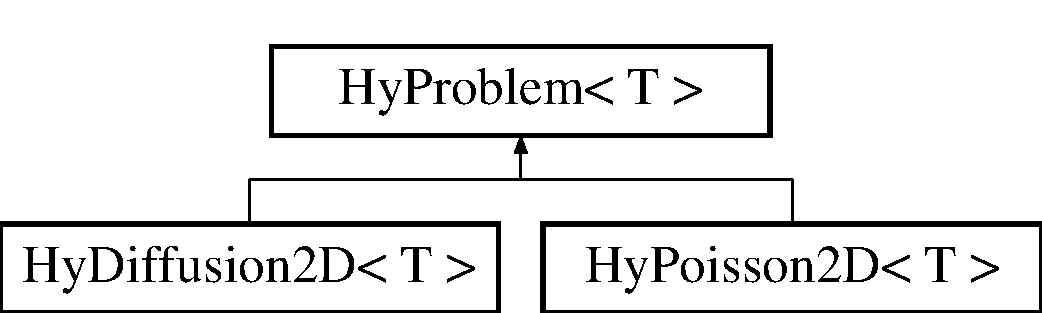
\includegraphics[height=2cm]{classHyProblem}
\end{center}
\end{figure}
\subsection*{Public Member Functions}
\begin{DoxyCompactItemize}
\item 
\hypertarget{classHyProblem_adc400712e624ef7107837a200082106a}{
\hyperlink{classHyProblem_adc400712e624ef7107837a200082106a}{HyProblem} ()}
\label{classHyProblem_adc400712e624ef7107837a200082106a}

\begin{DoxyCompactList}\small\item\em Default constructor. \item\end{DoxyCompactList}\item 
\hypertarget{classHyProblem_a7095777a5ace089bc97b94dca99b15e5}{
{\bfseries HyProblem} (\hyperlink{classHyDomain}{HyDomain}$<$ T $>$ \&pDomain, \hyperlink{classHyBoundary}{HyBoundary}$<$ T $>$ \&pBoundary, \hyperlink{classHyMesh2D}{HyMesh2D}$<$ T $>$ \&pMesh, std::string \&pDescription)}
\label{classHyProblem_a7095777a5ace089bc97b94dca99b15e5}

\item 
\hypertarget{classHyProblem_a83930a79d3e3129d9baccfc87dc5b644}{
\hyperlink{classHyBoundary}{HyBoundary}$<$ T $>$ \& {\bfseries getBoundary} ()}
\label{classHyProblem_a83930a79d3e3129d9baccfc87dc5b644}

\item 
\hypertarget{classHyProblem_a11d299a8fb714521e9372e9c52c83624}{
std::string \& {\bfseries getDescription} ()}
\label{classHyProblem_a11d299a8fb714521e9372e9c52c83624}

\item 
\hypertarget{classHyProblem_a5afc0faab283a084c4362789089300fa}{
\hyperlink{classHyDomain}{HyDomain}$<$ T $>$ \& {\bfseries getDomain} ()}
\label{classHyProblem_a5afc0faab283a084c4362789089300fa}

\item 
\hypertarget{classHyProblem_aa0d4e2347207b2e81aba21ff71d2d466}{
\hyperlink{classHyMesh2D}{HyMesh2D}$<$ T $>$ \& {\bfseries getMesh} ()}
\label{classHyProblem_aa0d4e2347207b2e81aba21ff71d2d466}

\item 
\hypertarget{classHyProblem_a69ec82f40bcde905ae9bed9b181680fe}{
Eigen::SparseMatrix$<$ T $>$ \& {\bfseries getMatrix} ()}
\label{classHyProblem_a69ec82f40bcde905ae9bed9b181680fe}

\item 
\hypertarget{classHyProblem_a7fc4251c8a28039d5fc1e954420b9e8d}{
Eigen::VectorXd \& {\bfseries getX} ()}
\label{classHyProblem_a7fc4251c8a28039d5fc1e954420b9e8d}

\item 
\hypertarget{classHyProblem_a8ebd85b6c5c13d94d9f8be8041ca2507}{
Eigen::VectorXd \& {\bfseries getF} ()}
\label{classHyProblem_a8ebd85b6c5c13d94d9f8be8041ca2507}

\item 
\hypertarget{classHyProblem_a2024a50f38fd285fc60eb88a549094cb}{
Eigen::VectorXd \& {\bfseries getG} ()}
\label{classHyProblem_a2024a50f38fd285fc60eb88a549094cb}

\item 
\hypertarget{classHyProblem_abdd44294731eb686dcd5254ef7bafe74}{
void {\bfseries setBoundary} (\hyperlink{classHyBoundary}{HyBoundary}$<$ T $>$ \&lB)}
\label{classHyProblem_abdd44294731eb686dcd5254ef7bafe74}

\item 
\hypertarget{classHyProblem_ae7feccde80b8a6db481908b70d6eb24e}{
void {\bfseries setX} (Eigen::VectorXd pVector)}
\label{classHyProblem_ae7feccde80b8a6db481908b70d6eb24e}

\item 
\hypertarget{classHyProblem_a6419ca29465c86cc742efd7dba79f1b3}{
virtual void {\bfseries build} ()=0}
\label{classHyProblem_a6419ca29465c86cc742efd7dba79f1b3}

\item 
void \hyperlink{classHyProblem_a894b6467b03798221e48e1fb10ad3fcf}{updateMesh} ()
\begin{DoxyCompactList}\small\item\em Check if each point is inside the domain Omega, on the boundary, or outside. Also update neighbourhood. \item\end{DoxyCompactList}\item 
\hypertarget{classHyProblem_a4f5e62e3412d2e7b1475a8ec6a44052a}{
virtual void {\bfseries solve} ()=0}
\label{classHyProblem_a4f5e62e3412d2e7b1475a8ec6a44052a}

\item 
double \hyperlink{classHyProblem_a5d3b78c69811136e74e9fc9232cc110b}{g} (\hyperlink{classHyPoint}{HyPoint}$<$ T $>$ pPoint)
\begin{DoxyCompactList}\small\item\em The Dirichlet condition on the boundary. \item\end{DoxyCompactList}\item 
\hypertarget{classHyProblem_a14a8e72160ffe2e90664c40a53930c54}{
double {\bfseries g} (T pX, T pY, T pZ)}
\label{classHyProblem_a14a8e72160ffe2e90664c40a53930c54}

\item 
\hypertarget{classHyProblem_a35ab1f86f6069adcfc9d2d958a6181b9}{
void \hyperlink{classHyProblem_a35ab1f86f6069adcfc9d2d958a6181b9}{display} (std::ostream \&out)}
\label{classHyProblem_a35ab1f86f6069adcfc9d2d958a6181b9}

\begin{DoxyCompactList}\small\item\em Displays the object HyProblem2D. \item\end{DoxyCompactList}\item 
\hypertarget{classHyProblem_a826f04877aef38225f7661b37969f946}{
void {\bfseries displaySolutionGP} (std::ostream \&out)}
\label{classHyProblem_a826f04877aef38225f7661b37969f946}

\item 
\hypertarget{classHyProblem_a77b1843d7ea8271849e7d3d804587c12}{
\hyperlink{classHyProblem}{HyProblem}$<$ T $>$ \& {\bfseries operator=} (const \hyperlink{classHyProblem}{HyProblem}$<$ T $>$ \&pP)}
\label{classHyProblem_a77b1843d7ea8271849e7d3d804587c12}

\end{DoxyCompactItemize}
\subsection*{Protected Attributes}
\begin{DoxyCompactItemize}
\item 
\hyperlink{classHyDomain}{HyDomain}$<$ T $>$ \& \hyperlink{classHyProblem_a245270926a69fef2df91e3aad939fee3}{aDomain}
\item 
\hyperlink{classHyBoundary}{HyBoundary}$<$ T $>$ \& \hyperlink{classHyProblem_af7a46447af3592758cb384ac355a30fd}{aBoundary}
\item 
\hyperlink{classHyMesh2D}{HyMesh2D}$<$ T $>$ \& \hyperlink{classHyProblem_a370a94346e3e688f352f60ff1e8ba1ab}{aMesh}
\item 
std::string \& \hyperlink{classHyProblem_a9ff58aa13598c448222203cbb0ad6a10}{aDescription}
\item 
Eigen::SparseMatrix$<$ T $>$ \hyperlink{classHyProblem_a4930e5e04c383d64f8a3eb2dfe24fb54}{aMatrix}
\item 
Eigen::VectorXd \hyperlink{classHyProblem_ad08883fb8ad06aadda0302fc387433cf}{aX}
\item 
Eigen::VectorXd \hyperlink{classHyProblem_a9c31ddb647141522c68ce12c1fc0036b}{aF}
\item 
Eigen::VectorXd \hyperlink{classHyProblem_a3426083f6fd97b687b72b6656db0a224}{aG}
\end{DoxyCompactItemize}


\subsection{Detailed Description}
\subsubsection*{template$<$typename T$>$ class HyProblem$<$ T $>$}

Defines a physical problem. The class \hyperlink{classHyProblem}{HyProblem} represents a physical problem described by a domain, its boundary, the corresponding PDE and the boundary conditions. The numerical solution is obtained by solving the linear system AX = F+G. A represents the matrix (determined by the equation of the problem), X is the unknown vector (the approximate solution), F 

\subsection{Member Function Documentation}
\hypertarget{classHyProblem_a5d3b78c69811136e74e9fc9232cc110b}{
\index{HyProblem@{HyProblem}!g@{g}}
\index{g@{g}!HyProblem@{HyProblem}}
\subsubsection[{g}]{\setlength{\rightskip}{0pt plus 5cm}template$<$typename T $>$ double {\bf HyProblem}$<$ T $>$::g ({\bf HyPoint}$<$ T $>$ {\em pPoint})\hspace{0.3cm}{\ttfamily  \mbox{[}inline\mbox{]}}}}
\label{classHyProblem_a5d3b78c69811136e74e9fc9232cc110b}


The Dirichlet condition on the boundary. 


\begin{DoxyParams}{Parameters}
\item[{\em pPoint}]The point of evaluation \end{DoxyParams}
\begin{DoxyReturn}{Returns}
The value of the Dirichlet condition on pPoint 
\end{DoxyReturn}


Reimplemented in \hyperlink{classHyDiffusion2D_a0df1a7fbe0b6a50d85a74c655f32cfb2}{HyDiffusion2D$<$ T $>$}, and \hyperlink{classHyPoisson2D_a9c27e90e3abb3a6ebe5d6b3274412e7a}{HyPoisson2D$<$ T $>$}.

\hypertarget{classHyProblem_a894b6467b03798221e48e1fb10ad3fcf}{
\index{HyProblem@{HyProblem}!updateMesh@{updateMesh}}
\index{updateMesh@{updateMesh}!HyProblem@{HyProblem}}
\subsubsection[{updateMesh}]{\setlength{\rightskip}{0pt plus 5cm}template$<$typename T $>$ void {\bf HyProblem}$<$ T $>$::updateMesh ()\hspace{0.3cm}{\ttfamily  \mbox{[}inline\mbox{]}}}}
\label{classHyProblem_a894b6467b03798221e48e1fb10ad3fcf}


Check if each point is inside the domain Omega, on the boundary, or outside. Also update neighbourhood. 


\begin{DoxyParams}{Parameters}
\item[{\em pPoint}]The point of evaluation \end{DoxyParams}
\begin{DoxyReturn}{Returns}
The value of the Dirichlet condition on pPoint 
\end{DoxyReturn}


\subsection{Member Data Documentation}
\hypertarget{classHyProblem_af7a46447af3592758cb384ac355a30fd}{
\index{HyProblem@{HyProblem}!aBoundary@{aBoundary}}
\index{aBoundary@{aBoundary}!HyProblem@{HyProblem}}
\subsubsection[{aBoundary}]{\setlength{\rightskip}{0pt plus 5cm}template$<$typename T$>$ {\bf HyBoundary}$<$T$>$\& {\bf HyProblem}$<$ T $>$::{\bf aBoundary}\hspace{0.3cm}{\ttfamily  \mbox{[}protected\mbox{]}}}}
\label{classHyProblem_af7a46447af3592758cb384ac355a30fd}
The boundary of the domain \hypertarget{classHyProblem_a9ff58aa13598c448222203cbb0ad6a10}{
\index{HyProblem@{HyProblem}!aDescription@{aDescription}}
\index{aDescription@{aDescription}!HyProblem@{HyProblem}}
\subsubsection[{aDescription}]{\setlength{\rightskip}{0pt plus 5cm}template$<$typename T$>$ std::string\& {\bf HyProblem}$<$ T $>$::{\bf aDescription}\hspace{0.3cm}{\ttfamily  \mbox{[}protected\mbox{]}}}}
\label{classHyProblem_a9ff58aa13598c448222203cbb0ad6a10}
A brief description of the problem \hypertarget{classHyProblem_a245270926a69fef2df91e3aad939fee3}{
\index{HyProblem@{HyProblem}!aDomain@{aDomain}}
\index{aDomain@{aDomain}!HyProblem@{HyProblem}}
\subsubsection[{aDomain}]{\setlength{\rightskip}{0pt plus 5cm}template$<$typename T$>$ {\bf HyDomain}$<$T$>$\& {\bf HyProblem}$<$ T $>$::{\bf aDomain}\hspace{0.3cm}{\ttfamily  \mbox{[}protected\mbox{]}}}}
\label{classHyProblem_a245270926a69fef2df91e3aad939fee3}
The whole rectangular domain that will determine the mesh \hypertarget{classHyProblem_a9c31ddb647141522c68ce12c1fc0036b}{
\index{HyProblem@{HyProblem}!aF@{aF}}
\index{aF@{aF}!HyProblem@{HyProblem}}
\subsubsection[{aF}]{\setlength{\rightskip}{0pt plus 5cm}template$<$typename T$>$ Eigen::VectorXd {\bf HyProblem}$<$ T $>$::{\bf aF}\hspace{0.3cm}{\ttfamily  \mbox{[}protected\mbox{]}}}}
\label{classHyProblem_a9c31ddb647141522c68ce12c1fc0036b}
The vector containing values of the f function \hypertarget{classHyProblem_a3426083f6fd97b687b72b6656db0a224}{
\index{HyProblem@{HyProblem}!aG@{aG}}
\index{aG@{aG}!HyProblem@{HyProblem}}
\subsubsection[{aG}]{\setlength{\rightskip}{0pt plus 5cm}template$<$typename T$>$ Eigen::VectorXd {\bf HyProblem}$<$ T $>$::{\bf aG}\hspace{0.3cm}{\ttfamily  \mbox{[}protected\mbox{]}}}}
\label{classHyProblem_a3426083f6fd97b687b72b6656db0a224}
The vector containing values of the Dirichlet condition \hypertarget{classHyProblem_a4930e5e04c383d64f8a3eb2dfe24fb54}{
\index{HyProblem@{HyProblem}!aMatrix@{aMatrix}}
\index{aMatrix@{aMatrix}!HyProblem@{HyProblem}}
\subsubsection[{aMatrix}]{\setlength{\rightskip}{0pt plus 5cm}template$<$typename T$>$ Eigen::SparseMatrix$<$T$>$ {\bf HyProblem}$<$ T $>$::{\bf aMatrix}\hspace{0.3cm}{\ttfamily  \mbox{[}protected\mbox{]}}}}
\label{classHyProblem_a4930e5e04c383d64f8a3eb2dfe24fb54}
The matrix A of the linear problem \hypertarget{classHyProblem_a370a94346e3e688f352f60ff1e8ba1ab}{
\index{HyProblem@{HyProblem}!aMesh@{aMesh}}
\index{aMesh@{aMesh}!HyProblem@{HyProblem}}
\subsubsection[{aMesh}]{\setlength{\rightskip}{0pt plus 5cm}template$<$typename T$>$ {\bf HyMesh2D}$<$T$>$\& {\bf HyProblem}$<$ T $>$::{\bf aMesh}\hspace{0.3cm}{\ttfamily  \mbox{[}protected\mbox{]}}}}
\label{classHyProblem_a370a94346e3e688f352f60ff1e8ba1ab}
The mesh for the numerical resolution \hypertarget{classHyProblem_ad08883fb8ad06aadda0302fc387433cf}{
\index{HyProblem@{HyProblem}!aX@{aX}}
\index{aX@{aX}!HyProblem@{HyProblem}}
\subsubsection[{aX}]{\setlength{\rightskip}{0pt plus 5cm}template$<$typename T$>$ Eigen::VectorXd {\bf HyProblem}$<$ T $>$::{\bf aX}\hspace{0.3cm}{\ttfamily  \mbox{[}protected\mbox{]}}}}
\label{classHyProblem_ad08883fb8ad06aadda0302fc387433cf}
The unknown solution 

The documentation for this class was generated from the following files:\begin{DoxyCompactItemize}
\item 
\hyperlink{HyProblem_8hpp}{HyProblem.hpp}\item 
\hyperlink{HyProblem_8ipp}{HyProblem.ipp}\end{DoxyCompactItemize}

\hypertarget{classHyRectangle}{
\section{HyRectangle$<$ T $>$ Class Template Reference}
\label{classHyRectangle}\index{HyRectangle@{HyRectangle}}
}
Inheritance diagram for HyRectangle$<$ T $>$:\begin{figure}[H]
\begin{center}
\leavevmode
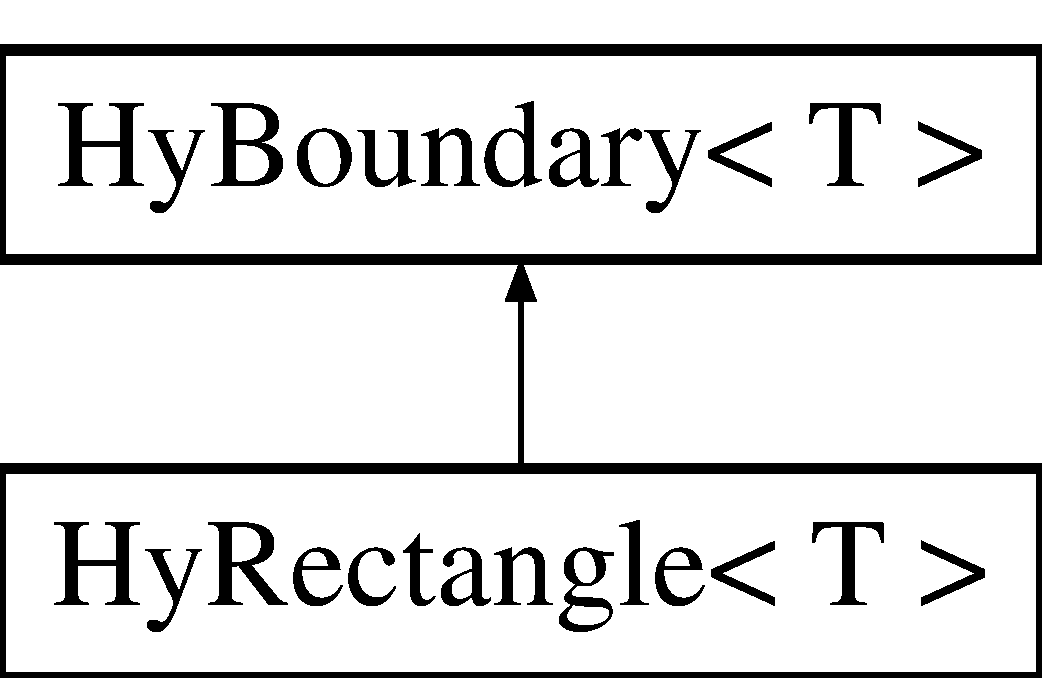
\includegraphics[height=2cm]{classHyRectangle}
\end{center}
\end{figure}
\subsection*{Public Member Functions}
\begin{DoxyCompactItemize}
\item 
\hypertarget{classHyRectangle_afab85331b1158d1215bac7680e67a456}{
{\bfseries HyRectangle} (\hyperlink{classHyPoint}{HyPoint}$<$ T $>$ \&pBL, \hyperlink{classHyPoint}{HyPoint}$<$ T $>$ \&pUR)}
\label{classHyRectangle_afab85331b1158d1215bac7680e67a456}

\item 
\hypertarget{classHyRectangle_a8a81ae18b51a5580752d524e8f17a4f7}{
\hyperlink{classHyPoint}{HyPoint}$<$ T $>$ \& {\bfseries getBL} ()}
\label{classHyRectangle_a8a81ae18b51a5580752d524e8f17a4f7}

\item 
\hypertarget{classHyRectangle_a49e7757b39e6210905cb82d04b340b0e}{
\hyperlink{classHyPoint}{HyPoint}$<$ T $>$ \& {\bfseries getUR} ()}
\label{classHyRectangle_a49e7757b39e6210905cb82d04b340b0e}

\item 
\hypertarget{classHyRectangle_a615ce12bfbb99d0f83df522e42d83a8d}{
void {\bfseries setBL} (\hyperlink{classHyPoint}{HyPoint}$<$ T $>$ \&pBL)}
\label{classHyRectangle_a615ce12bfbb99d0f83df522e42d83a8d}

\item 
\hypertarget{classHyRectangle_a9b6df049ea762af2fa4fceb5cc2e5750}{
void {\bfseries setUR} (\hyperlink{classHyPoint}{HyPoint}$<$ T $>$ \&pUR)}
\label{classHyRectangle_a9b6df049ea762af2fa4fceb5cc2e5750}

\item 
double \hyperlink{classHyRectangle_a881f7ed847a94d1af3ff4ff0d60ee516}{getBoundary} (\hyperlink{classHyPoint}{HyPoint}$<$ T $>$ \&pPoint)
\begin{DoxyCompactList}\small\item\em Definition of the boundary. Positive inside the domain, 0 on the boundary, negative outside. \item\end{DoxyCompactList}\item 
\hypertarget{classHyRectangle_a96f3c7b970fe67fdea44c2b8fd52cb4a}{
double {\bfseries getBoundary} (T pX, T pY, T pZ)}
\label{classHyRectangle_a96f3c7b970fe67fdea44c2b8fd52cb4a}

\end{DoxyCompactItemize}
\subsection*{Protected Attributes}
\begin{DoxyCompactItemize}
\item 
\hypertarget{classHyRectangle_a6558ec991eedf516873b99aecc128b9f}{
\hyperlink{classHyPoint}{HyPoint}$<$ T $>$ {\bfseries aBL}}
\label{classHyRectangle_a6558ec991eedf516873b99aecc128b9f}

\item 
\hypertarget{classHyRectangle_a2442aa3cd909f02ca86b4b3cf4c78e6b}{
\hyperlink{classHyPoint}{HyPoint}$<$ T $>$ {\bfseries aUR}}
\label{classHyRectangle_a2442aa3cd909f02ca86b4b3cf4c78e6b}

\end{DoxyCompactItemize}
\subsubsection*{template$<$typename T$>$ class HyRectangle$<$ T $>$}



\subsection{Member Function Documentation}
\hypertarget{classHyRectangle_a881f7ed847a94d1af3ff4ff0d60ee516}{
\index{HyRectangle@{HyRectangle}!getBoundary@{getBoundary}}
\index{getBoundary@{getBoundary}!HyRectangle@{HyRectangle}}
\subsubsection[{getBoundary}]{\setlength{\rightskip}{0pt plus 5cm}template$<$typename T $>$ double {\bf HyRectangle}$<$ T $>$::getBoundary ({\bf HyPoint}$<$ T $>$ \& {\em pPoint})\hspace{0.3cm}{\ttfamily  \mbox{[}inline\mbox{]}}}}
\label{classHyRectangle_a881f7ed847a94d1af3ff4ff0d60ee516}


Definition of the boundary. Positive inside the domain, 0 on the boundary, negative outside. 


\begin{DoxyParams}{Parameters}
\item[{\em pPoint}]The point to evalutate. \end{DoxyParams}


Reimplemented from \hyperlink{classHyBoundary_a138c96a97075dc41eead25963c1bf785}{HyBoundary$<$ T $>$}.



The documentation for this class was generated from the following files:\begin{DoxyCompactItemize}
\item 
HyRectangle.hpp\item 
HyRectangle.ipp\end{DoxyCompactItemize}

\hypertarget{classHySetPoints}{
\section{HySetPoints$<$ T $>$ Class Template Reference}
\label{classHySetPoints}\index{HySetPoints@{HySetPoints}}
}
\subsection*{Public Member Functions}
\begin{DoxyCompactItemize}
\item 
\hypertarget{classHySetPoints_a8ca08da4c53feebbaf3d2ca9903831ef}{
std::vector$<$ \hyperlink{classHyPoint}{HyPoint}$<$ T $>$ $\ast$ $>$ \& {\bfseries getSet} ()}
\label{classHySetPoints_a8ca08da4c53feebbaf3d2ca9903831ef}

\item 
\hypertarget{classHySetPoints_a127c51e7b1ea4712ab443b2f3479d88f}{
unsigned int {\bfseries size} ()}
\label{classHySetPoints_a127c51e7b1ea4712ab443b2f3479d88f}

\item 
\hypertarget{classHySetPoints_a99697790811a1c3f38cde3255810f62e}{
\hyperlink{classHyPoint}{HyPoint}$<$ T $>$ \& {\bfseries operator\mbox{[}$\,$\mbox{]}} (unsigned int i)}
\label{classHySetPoints_a99697790811a1c3f38cde3255810f62e}

\item 
\hypertarget{classHySetPoints_a64e34251bcc54b6b69e09b53691c7724}{
void {\bfseries add} (\hyperlink{classHyPoint}{HyPoint}$<$ T $>$ $\ast$pPoint)}
\label{classHySetPoints_a64e34251bcc54b6b69e09b53691c7724}

\item 
\hypertarget{classHySetPoints_afa41d38a489c9ee60b42d2d354cb48fb}{
void {\bfseries add} (\hyperlink{classHyPoint}{HyPoint}$<$ T $>$ \&pPoint)}
\label{classHySetPoints_afa41d38a489c9ee60b42d2d354cb48fb}

\end{DoxyCompactItemize}
\subsection*{Protected Attributes}
\begin{DoxyCompactItemize}
\item 
\hypertarget{classHySetPoints_a1c4d2f32fe0aeb85f1efb6aad3b23d44}{
std::vector$<$ \hyperlink{classHyPoint}{HyPoint}$<$ T $>$ $\ast$ $>$ {\bfseries aSet}}
\label{classHySetPoints_a1c4d2f32fe0aeb85f1efb6aad3b23d44}

\end{DoxyCompactItemize}
\subsubsection*{template$<$typename T$>$ class HySetPoints$<$ T $>$}



The documentation for this class was generated from the following files:\begin{DoxyCompactItemize}
\item 
HySetPoints.hpp\item 
HySetPoints.ipp\end{DoxyCompactItemize}

\hypertarget{classHySolver}{
\section{HySolver$<$ T $>$ Class Template Reference}
\label{classHySolver}\index{HySolver@{HySolver}}
}
\subsection*{Public Member Functions}
\begin{DoxyCompactItemize}
\item 
\hypertarget{classHySolver_ac31ba2f76607bc0de77b6477713bb0bf}{
void {\bfseries withBiCGSTAB} (\hyperlink{classHyProblem}{HyProblem}$<$ T $>$ \&pProblem)}
\label{classHySolver_ac31ba2f76607bc0de77b6477713bb0bf}

\item 
\hypertarget{classHySolver_ab84b7618d9913077db95a4abbc75b9ea}{
void {\bfseries withConjugateGradient} (\hyperlink{classHyProblem}{HyProblem}$<$ T $>$ \&pProblem)}
\label{classHySolver_ab84b7618d9913077db95a4abbc75b9ea}

\end{DoxyCompactItemize}
\subsection*{Protected Attributes}
\begin{DoxyCompactItemize}
\item 
\hypertarget{classHySolver_a2114866d91c7c48ce5100fefb3086c5e}{
double {\bfseries aError}}
\label{classHySolver_a2114866d91c7c48ce5100fefb3086c5e}

\end{DoxyCompactItemize}
\subsubsection*{template$<$typename T$>$ class HySolver$<$ T $>$}



The documentation for this class was generated from the following files:\begin{DoxyCompactItemize}
\item 
HySolver.hpp\item 
HySolver.ipp\end{DoxyCompactItemize}

\chapter{File Documentation}
\hypertarget{HyBoundary_8hpp}{
\section{HyBoundary.hpp File Reference}
\label{HyBoundary_8hpp}\index{HyBoundary.hpp@{HyBoundary.hpp}}
}


Header file of \hyperlink{classHyBoundary}{HyBoundary} class.  


{\ttfamily \#include $<$string$>$}\par
{\ttfamily \#include \char`\"{}HyDomain.hpp\char`\"{}}\par
{\ttfamily \#include $<$cmath$>$}\par
{\ttfamily \#include $<$iostream$>$}\par
{\ttfamily \#include \char`\"{}HyDomain.hpp\char`\"{}}\par
{\ttfamily \#include \char`\"{}HyPoint.hpp\char`\"{}}\par
\subsection*{Classes}
\begin{DoxyCompactItemize}
\item 
class \hyperlink{classHyBoundary}{HyBoundary$<$ T $>$}
\begin{DoxyCompactList}\small\item\em Define the border of the domain for a given problem. It is represented by a function, defined in the whole space, which value is positive inside the domain, 0 exactly on the boundary, and negative outside. This class is virtual. \item\end{DoxyCompactList}\end{DoxyCompactItemize}
\subsection*{Functions}
\begin{DoxyCompactItemize}
\item 
{\footnotesize template$<$typename T $>$ }\\std::ostream \& \hyperlink{HyBoundary_8hpp_ac68022df35a83e2f5c37f203d801ba05}{operator$<$$<$} (std::ostream \&out, \hyperlink{classHyBoundary}{HyBoundary}$<$ T $>$ pBound)
\begin{DoxyCompactList}\small\item\em operator$<$$<$ \item\end{DoxyCompactList}\end{DoxyCompactItemize}


\subsection{Detailed Description}
Header file of \hyperlink{classHyBoundary}{HyBoundary} class. 

\subsection{Function Documentation}
\hypertarget{HyBoundary_8hpp_ac68022df35a83e2f5c37f203d801ba05}{
\index{HyBoundary.hpp@{HyBoundary.hpp}!operator$<$$<$@{operator$<$$<$}}
\index{operator$<$$<$@{operator$<$$<$}!HyBoundary.hpp@{HyBoundary.hpp}}
\subsubsection[{operator$<$$<$}]{\setlength{\rightskip}{0pt plus 5cm}template$<$typename T $>$ std::ostream \& operator$<$$<$ (std::ostream \& {\em out}, \/  {\bf HyBoundary}$<$ T $>$ {\em pBound})\hspace{0.3cm}{\ttfamily  \mbox{[}inline\mbox{]}}}}
\label{HyBoundary_8hpp_ac68022df35a83e2f5c37f203d801ba05}


operator$<$$<$ 


\begin{DoxyParams}{Parameters}
\item[{\em out}]The ostream to write in. \item[{\em pBound}]The \hyperlink{classHyBoundary}{HyBoundary} to display. \end{DoxyParams}

\hypertarget{HyBoundary_8ipp}{
\section{HyBoundary.ipp File Reference}
\label{HyBoundary_8ipp}\index{HyBoundary.ipp@{HyBoundary.ipp}}
}


Template file of \hyperlink{classHyBoundary}{HyBoundary} class.  


\subsection*{Functions}
\begin{DoxyCompactItemize}
\item 
{\footnotesize template$<$typename T $>$ }\\std::ostream \& \hyperlink{HyBoundary_8ipp_aa17bace639b97b7cdc5fa104cd3d7189}{operator$<$$<$} (std::ostream \&out, \hyperlink{classHyBoundary}{HyBoundary}$<$ T $>$ pBound)
\begin{DoxyCompactList}\small\item\em operator$<$$<$ \item\end{DoxyCompactList}\end{DoxyCompactItemize}


\subsection{Detailed Description}
Template file of \hyperlink{classHyBoundary}{HyBoundary} class. 

\subsection{Function Documentation}
\hypertarget{HyBoundary_8ipp_aa17bace639b97b7cdc5fa104cd3d7189}{
\index{HyBoundary.ipp@{HyBoundary.ipp}!operator$<$$<$@{operator$<$$<$}}
\index{operator$<$$<$@{operator$<$$<$}!HyBoundary.ipp@{HyBoundary.ipp}}
\subsubsection[{operator$<$$<$}]{\setlength{\rightskip}{0pt plus 5cm}template$<$typename T $>$ std::ostream\& operator$<$$<$ (std::ostream \& {\em out}, \/  {\bf HyBoundary}$<$ T $>$ {\em pBound})\hspace{0.3cm}{\ttfamily  \mbox{[}inline\mbox{]}}}}
\label{HyBoundary_8ipp_aa17bace639b97b7cdc5fa104cd3d7189}


operator$<$$<$ 


\begin{DoxyParams}{Parameters}
\item[{\em out}]The ostream to write in. \item[{\em pBound}]The \hyperlink{classHyBoundary}{HyBoundary} to display. \end{DoxyParams}

\hypertarget{HyDiffusion2D_8hpp}{
\section{HyDiffusion2D.hpp File Reference}
\label{HyDiffusion2D_8hpp}\index{HyDiffusion2D.hpp@{HyDiffusion2D.hpp}}
}


Header file of \hyperlink{classHyDiffusion2D}{HyDiffusion2D} class.  


{\ttfamily \#include $<$string$>$}\par
{\ttfamily \#include \char`\"{}HyBoundary.hpp\char`\"{}}\par
{\ttfamily \#include \char`\"{}HyMesh2D.hpp\char`\"{}}\par
{\ttfamily \#include $<$iostream$>$}\par
{\ttfamily \#include $<$vector$>$}\par
{\ttfamily \#include \char`\"{}HyPoint.hpp\char`\"{}}\par
{\ttfamily \#include \char`\"{}Variables.hpp\char`\"{}}\par
{\ttfamily \#include \char`\"{}HyMesh2D.hpp\char`\"{}}\par
{\ttfamily \#include \char`\"{}HyProblem.hpp\char`\"{}}\par
{\ttfamily \#include \char`\"{}HyDomain.hpp\char`\"{}}\par
{\ttfamily \#include $<$Eigen/Sparse$>$}\par
\subsection*{Classes}
\begin{DoxyCompactItemize}
\item 
class \hyperlink{classHyDiffusion2D}{HyDiffusion2D$<$ T $>$}
\begin{DoxyCompactList}\small\item\em Diffusion equation in 2 dimensions: $ \partial_t u - \kappa\Delta u = f $. \item\end{DoxyCompactList}\end{DoxyCompactItemize}
\subsection*{Functions}
\begin{DoxyCompactItemize}
\item 
\hypertarget{HyDiffusion2D_8hpp_ad454ede8ddfc399c5ef2ff927862a329}{
{\footnotesize template$<$typename T $>$ }\\std::ostream \& {\bfseries operator$<$$<$} (std::ostream \&out, \hyperlink{classHyDiffusion2D}{HyDiffusion2D}$<$ T $>$ pProb)}
\label{HyDiffusion2D_8hpp_ad454ede8ddfc399c5ef2ff927862a329}

\end{DoxyCompactItemize}


\subsection{Detailed Description}
Header file of \hyperlink{classHyDiffusion2D}{HyDiffusion2D} class. 
\hypertarget{HyDiffusion2D_8ipp}{
\section{HyDiffusion2D.ipp File Reference}
\label{HyDiffusion2D_8ipp}\index{HyDiffusion2D.ipp@{HyDiffusion2D.ipp}}
}


Template file of \hyperlink{classHyDiffusion2D}{HyDiffusion2D} class.  




\subsection{Detailed Description}
Template file of \hyperlink{classHyDiffusion2D}{HyDiffusion2D} class. 
\hypertarget{HyMesh1D_8hpp}{
\section{HyMesh1D.hpp File Reference}
\label{HyMesh1D_8hpp}\index{HyMesh1D.hpp@{HyMesh1D.hpp}}
}
{\ttfamily \#include $<$iostream$>$}\par
{\ttfamily \#include $<$vector$>$}\par
{\ttfamily \#include \char`\"{}HyMesh.hpp\char`\"{}}\par
{\ttfamily \#include \char`\"{}Variables.hpp\char`\"{}}\par
{\ttfamily \#include \char`\"{}HyMesh1D.ipp\char`\"{}}\par
{\ttfamily \#include \char`\"{}HyPoint.hpp\char`\"{}}\par
\subsection*{Classes}
\begin{DoxyCompactItemize}
\item 
class \hyperlink{classHyMesh1D}{HyMesh1D$<$ T $>$}
\end{DoxyCompactItemize}
\subsection*{Functions}
\begin{DoxyCompactItemize}
\item 
\hypertarget{HyMesh1D_8hpp_a710f53429fecad545abae64521bd5999}{
{\footnotesize template$<$typename T $>$ }\\std::ostream \& {\bfseries operator$<$$<$} (std::ostream \&out, \hyperlink{classHyMesh1D}{HyMesh1D}$<$ T $>$ \&pM)}
\label{HyMesh1D_8hpp_a710f53429fecad545abae64521bd5999}

\end{DoxyCompactItemize}


\subsection{Detailed Description}
\begin{DoxyDate}{Date}
2010
\end{DoxyDate}
Header of \hyperlink{classHyMesh1D}{HyMesh1D} class. Represents a cartesian 1D mesh. 
\hypertarget{HyMesh2D_8hpp}{
\section{HyMesh2D.hpp File Reference}
\label{HyMesh2D_8hpp}\index{HyMesh2D.hpp@{HyMesh2D.hpp}}
}
{\ttfamily \#include $<$iostream$>$}\par
{\ttfamily \#include $<$vector$>$}\par
{\ttfamily \#include \char`\"{}HyMesh.hpp\char`\"{}}\par
{\ttfamily \#include \char`\"{}Variables.hpp\char`\"{}}\par
{\ttfamily \#include \char`\"{}HyMesh2D.ipp\char`\"{}}\par
\subsection*{Classes}
\begin{DoxyCompactItemize}
\item 
class \hyperlink{classHyMesh2D}{HyMesh2D$<$ T $>$}
\begin{DoxyCompactList}\small\item\em Two dimensional mesh. \item\end{DoxyCompactList}\end{DoxyCompactItemize}
\subsection*{Functions}
\begin{DoxyCompactItemize}
\item 
\hypertarget{HyMesh2D_8hpp_ad4189be01196891b07dc91e75ede6466}{
{\footnotesize template$<$typename T $>$ }\\std::ostream \& \hyperlink{HyMesh2D_8hpp_ad4189be01196891b07dc91e75ede6466}{operator$<$$<$} (std::ostream \&out, \hyperlink{classHyMesh2D}{HyMesh2D}$<$ T $>$ \&pM)}
\label{HyMesh2D_8hpp_ad4189be01196891b07dc91e75ede6466}

\begin{DoxyCompactList}\small\item\em operator$<$$<$ \item\end{DoxyCompactList}\end{DoxyCompactItemize}


\subsection{Detailed Description}
\begin{DoxyDate}{Date}
2010
\end{DoxyDate}
Header of \hyperlink{classHyMesh2D}{HyMesh2D} class. Represents a cartesian 2D mesh. 
\hypertarget{HyPlotter_8hpp}{
\section{HyPlotter.hpp File Reference}
\label{HyPlotter_8hpp}\index{HyPlotter.hpp@{HyPlotter.hpp}}
}


Header file of \hyperlink{classHyPlotter}{HyPlotter} class.  


{\ttfamily \#include $<$iostream$>$}\par
{\ttfamily \#include $<$fstream$>$}\par
{\ttfamily \#include $<$sstream$>$}\par
{\ttfamily \#include $<$Eigen/Dense$>$}\par
{\ttfamily \#include \char`\"{}HyMesh2D.hpp\char`\"{}}\par
{\ttfamily \#include \char`\"{}HyPlotter.ipp\char`\"{}}\par
\subsection*{Classes}
\begin{DoxyCompactItemize}
\item 
class \hyperlink{classHyPlotter}{HyPlotter$<$ T $>$}
\end{DoxyCompactItemize}


\subsection{Detailed Description}
Header file of \hyperlink{classHyPlotter}{HyPlotter} class. 
\hypertarget{HyPoint_8hpp}{
\section{HyPoint.hpp File Reference}
\label{HyPoint_8hpp}\index{HyPoint.hpp@{HyPoint.hpp}}
}
{\ttfamily \#include $<$cmath$>$}\par
{\ttfamily \#include $<$iostream$>$}\par
{\ttfamily \#include \char`\"{}Variables.hpp\char`\"{}}\par
{\ttfamily \#include \char`\"{}HyPoint.ipp\char`\"{}}\par
\subsection*{Classes}
\begin{DoxyCompactItemize}
\item 
class \hyperlink{classHyPoint}{HyPoint$<$ T $>$}
\end{DoxyCompactItemize}
\subsection*{Functions}
\begin{DoxyCompactItemize}
\item 
\hypertarget{HyPoint_8hpp_a0ea4d4f73eca4379ca501510f23f548e}{
{\footnotesize template$<$typename T $>$ }\\\hyperlink{classHyPoint}{HyPoint}$<$ T $>$ {\bfseries operator+} (\hyperlink{classHyPoint}{HyPoint}$<$ T $>$ const \&pA, \hyperlink{classHyPoint}{HyPoint}$<$ T $>$ const \&pB)}
\label{HyPoint_8hpp_a0ea4d4f73eca4379ca501510f23f548e}

\item 
\hypertarget{HyPoint_8hpp_ad84a14d9043ae9aada8c8210b876a28c}{
{\footnotesize template$<$typename T $>$ }\\\hyperlink{classHyPoint}{HyPoint}$<$ T $>$ {\bfseries operator/} (\hyperlink{classHyPoint}{HyPoint}$<$ T $>$ const \&pA, double pX)}
\label{HyPoint_8hpp_ad84a14d9043ae9aada8c8210b876a28c}

\item 
\hypertarget{HyPoint_8hpp_a61dbecdfd1a22686296889727a037e4b}{
{\footnotesize template$<$typename T $>$ }\\std::ostream \& {\bfseries operator$<$$<$} (std::ostream \&pOut, \hyperlink{classHyPoint}{HyPoint}$<$ T $>$ \&pP)}
\label{HyPoint_8hpp_a61dbecdfd1a22686296889727a037e4b}

\end{DoxyCompactItemize}


\subsection{Detailed Description}
\begin{DoxyAuthor}{Author}
Hybryd-\/ 
\end{DoxyAuthor}
\begin{DoxyDate}{Date}
2010
\end{DoxyDate}
Header of \hyperlink{classHyPoint}{HyPoint} class 
\hypertarget{HyPoisson2D_8hpp}{
\section{HyPoisson2D.hpp File Reference}
\label{HyPoisson2D_8hpp}\index{HyPoisson2D.hpp@{HyPoisson2D.hpp}}
}


Header file of \hyperlink{classHyPoisson2D}{HyPoisson2D} class.  


{\ttfamily \#include $<$string$>$}\par
{\ttfamily \#include \char`\"{}HyBoundary.hpp\char`\"{}}\par
{\ttfamily \#include \char`\"{}HyMesh2D.hpp\char`\"{}}\par
{\ttfamily \#include \char`\"{}HyProblem.hpp\char`\"{}}\par
{\ttfamily \#include \char`\"{}HyPoisson2D.ipp\char`\"{}}\par
\subsection*{Classes}
\begin{DoxyCompactItemize}
\item 
class \hyperlink{classHyPoisson2D}{HyPoisson2D$<$ T $>$}
\begin{DoxyCompactList}\small\item\em Poisson equation in 2 dimensions: $ \Delta u = f $. \item\end{DoxyCompactList}\end{DoxyCompactItemize}
\subsection*{Functions}
\begin{DoxyCompactItemize}
\item 
\hypertarget{HyPoisson2D_8hpp_a58836638cad8aae6143c66a2e3a6088e}{
{\footnotesize template$<$typename T $>$ }\\std::ostream \& {\bfseries operator$<$$<$} (std::ostream \&out, \hyperlink{classHyPoisson2D}{HyPoisson2D}$<$ T $>$ pProb)}
\label{HyPoisson2D_8hpp_a58836638cad8aae6143c66a2e3a6088e}

\end{DoxyCompactItemize}


\subsection{Detailed Description}
Header file of \hyperlink{classHyPoisson2D}{HyPoisson2D} class. 
\hypertarget{HyPoisson2D_8ipp}{
\section{HyPoisson2D.ipp File Reference}
\label{HyPoisson2D_8ipp}\index{HyPoisson2D.ipp@{HyPoisson2D.ipp}}
}


Template file of \hyperlink{classHyPoisson2D}{HyPoisson2D} class.  




\subsection{Detailed Description}
Template file of \hyperlink{classHyPoisson2D}{HyPoisson2D} class. 
\hypertarget{HyProblem_8hpp}{
\section{HyProblem.hpp File Reference}
\label{HyProblem_8hpp}\index{HyProblem.hpp@{HyProblem.hpp}}
}


Header file of \hyperlink{classHyProblem}{HyProblem} class.  


{\ttfamily \#include $<$iostream$>$}\par
{\ttfamily \#include $<$string$>$}\par
{\ttfamily \#include \char`\"{}HyBoundary.hpp\char`\"{}}\par
{\ttfamily \#include \char`\"{}HyMesh2D.hpp\char`\"{}}\par
{\ttfamily \#include \char`\"{}HyProblem.hpp\char`\"{}}\par
{\ttfamily \#include \char`\"{}HyDomain.hpp\char`\"{}}\par
{\ttfamily \#include $<$Eigen/Sparse$>$}\par
{\ttfamily \#include \char`\"{}HyProblem.ipp\char`\"{}}\par
\subsection*{Classes}
\begin{DoxyCompactItemize}
\item 
class \hyperlink{classHyProblem}{HyProblem$<$ T $>$}
\begin{DoxyCompactList}\small\item\em Defines a physical problem. \item\end{DoxyCompactList}\end{DoxyCompactItemize}
\subsection*{Functions}
\begin{DoxyCompactItemize}
\item 
\hypertarget{HyProblem_8hpp_a20eb81de73120dd950c0635ecc3ba698}{
{\footnotesize template$<$typename T $>$ }\\std::ostream \& \hyperlink{HyProblem_8hpp_a20eb81de73120dd950c0635ecc3ba698}{operator$<$$<$} (std::ostream \&out, \hyperlink{classHyProblem}{HyProblem}$<$ T $>$ pProb)}
\label{HyProblem_8hpp_a20eb81de73120dd950c0635ecc3ba698}

\begin{DoxyCompactList}\small\item\em Operator$<$$<$. \item\end{DoxyCompactList}\end{DoxyCompactItemize}


\subsection{Detailed Description}
Header file of \hyperlink{classHyProblem}{HyProblem} class. 
\hypertarget{HyProblem_8ipp}{
\section{HyProblem.ipp File Reference}
\label{HyProblem_8ipp}\index{HyProblem.ipp@{HyProblem.ipp}}
}


Template file of \hyperlink{classHyProblem}{HyProblem} class.  


\subsection*{Functions}
\begin{DoxyCompactItemize}
\item 
\hypertarget{HyProblem_8ipp_a8fd64b28fcc0373b7b3b045601bedc66}{
{\footnotesize template$<$typename T $>$ }\\std::ostream \& \hyperlink{HyProblem_8ipp_a8fd64b28fcc0373b7b3b045601bedc66}{operator$<$$<$} (std::ostream \&out, \hyperlink{classHyProblem}{HyProblem}$<$ T $>$ pProb)}
\label{HyProblem_8ipp_a8fd64b28fcc0373b7b3b045601bedc66}

\begin{DoxyCompactList}\small\item\em Operator$<$$<$. \item\end{DoxyCompactList}\end{DoxyCompactItemize}


\subsection{Detailed Description}
Template file of \hyperlink{classHyProblem}{HyProblem} class. 
\hypertarget{main_8cpp}{
\section{main.cpp File Reference}
\label{main_8cpp}\index{main.cpp@{main.cpp}}
}
{\ttfamily \#include $<$iostream$>$}\par
{\ttfamily \#include $<$fstream$>$}\par
{\ttfamily \#include $<$sstream$>$}\par
{\ttfamily \#include \char`\"{}HyMesh2D.hpp\char`\"{}}\par
{\ttfamily \#include \char`\"{}HyPoint.hpp\char`\"{}}\par
{\ttfamily \#include \char`\"{}HyPoisson2D.hpp\char`\"{}}\par
{\ttfamily \#include $<$string$>$}\par
{\ttfamily \#include \char`\"{}HyBoundary.hpp\char`\"{}}\par
{\ttfamily \#include \char`\"{}HyProblem.hpp\char`\"{}}\par
{\ttfamily \#include \char`\"{}HyPoisson2D.ipp\char`\"{}}\par
{\ttfamily \#include \char`\"{}HySolver.hpp\char`\"{}}\par
{\ttfamily \#include \char`\"{}HyDiffusion2D.ipp\char`\"{}}\par
{\ttfamily \#include $<$Eigen/Dense$>$}\par
{\ttfamily \#include \char`\"{}HyPlotter.ipp\char`\"{}}\par
{\ttfamily \#include \char`\"{}HyCircle.ipp\char`\"{}}\par
{\ttfamily \#include \char`\"{}HyRectangle.ipp\char`\"{}}\par
\subsection*{Functions}
\begin{DoxyCompactItemize}
\item 
\hypertarget{main_8cpp_a3c04138a5bfe5d72780bb7e82a18e627}{
int {\bfseries main} (int argc, char $\ast$$\ast$argv)}
\label{main_8cpp_a3c04138a5bfe5d72780bb7e82a18e627}

\end{DoxyCompactItemize}


\subsection{Detailed Description}
\begin{DoxyAuthor}{Author}
Hybryd-\/
\end{DoxyAuthor}
Numerical resolution of PDE using finite difference method 
\hypertarget{Variables_8hpp}{
\section{Variables.hpp File Reference}
\label{Variables_8hpp}\index{Variables.hpp@{Variables.hpp}}
}


List of all macros and parameters.  


\subsection*{Defines}
\begin{DoxyCompactItemize}
\item 
\hypertarget{Variables_8hpp_abfe67ba647fccb3e3fd38ab812af5c03}{
\#define {\bfseries DISPLAY\_\-MESH\_\-GRID\_\-STYLE}~1}
\label{Variables_8hpp_abfe67ba647fccb3e3fd38ab812af5c03}

\item 
\hypertarget{Variables_8hpp_a51671c3a712aacefed56c8af246b4800}{
\#define {\bfseries DISPLAY\_\-WHOLE\_\-MESH}~0}
\label{Variables_8hpp_a51671c3a712aacefed56c8af246b4800}

\item 
\hypertarget{Variables_8hpp_a0d355626c4aa97e77f0c69084baea147}{
\#define {\bfseries HY\_\-EPSILON}~0.000001}
\label{Variables_8hpp_a0d355626c4aa97e77f0c69084baea147}

\item 
\hypertarget{Variables_8hpp_ae9853b76880206c6a9c67d5f690b96a2}{
\#define {\bfseries HY\_\-PI}~3.1415926535}
\label{Variables_8hpp_ae9853b76880206c6a9c67d5f690b96a2}

\item 
\hypertarget{Variables_8hpp_a8ba5c0761794036a1968d3196205f705}{
\#define {\bfseries QUIET}~0}
\label{Variables_8hpp_a8ba5c0761794036a1968d3196205f705}

\end{DoxyCompactItemize}


\subsection{Detailed Description}
List of all macros and parameters. 
\begin{DoxyParams}{Parameters}
\item[{\em DISPLAY\_\-MESH\_\-GRID\_\-STYLE}]If the value is 1, displays the mesh like a grid in the terminal, with dots at each node. \item[{\em DISPLAY\_\-WHOLE\_\-MESH}]If the value is 1, displays the whole mesh (as a set of points). If 0, it only displays the domain defined by the \hyperlink{classHyBoundary}{HyBoundary}. It avoids displaying useless points outside the interesting domain. \item[{\em HY\_\-EPSILON}]Arbitrary precision, used in the code of this library only. \item[{\em HY\_\-PI}]Approximation of the most beautiful number of all the universe. \item[{\em QUIET}]If the value is 1, does not display any additionnal information like details of the problem or of the computation. \end{DoxyParams}

\printindex
\end{document}
